% Document releated
% \documentclass[12pt]{report}
\documentclass[12pt]{scrreprt}
\usepackage[utf8]{inputenc}
\usepackage[english]{babel}

% Configuration of KOMA-script
\setkomafont{dictumtext}{\itshape\small}
\setkomafont{dictumauthor}{\normalfont}
\renewcommand*\dictumwidth{0.75\linewidth}
\renewcommand*\dictumauthorformat[1]{\vspace{0.5cm}--- #1\vspace{0.25cm}}
\renewcommand*\dictumrule{}

% Cover configuration commands
\def\title#1{\gdef\@title{#1}\gdef\thetitle{#1}}
\def\subtitle#1{\gdef\@subtitle{#1}\gdef\thesubtitle{#1}}
\def\intro#1{\gdef\@intro{#1}\gdef\theintro{#1}}
\def\author#1{\gdef\@author{#1}\gdef\theauthor{#1}}
\def\meta#1{\gdef\@meta{#1}\gdef\themeta{#1}}

% Graphics
\usepackage{graphicx}
\usepackage{tikz}
\usepackage{float}

% Symbols and Math
\usepackage{amssymb}
\usepackage{amsmath}

% Code listings
\usepackage{listings}
\lstset{
  breaklines=true,
  basicstyle=\ttfamily
}
\lstset{columns=fullflexible,basicstyle=\ttfamily}
\usepackage{minted}

% References and links
\PassOptionsToPackage{hyphens}{url}\usepackage{hyperref}
\hypersetup{hidelinks=true}
\usepackage[usestackEOL]{stackengine}

% Custom tab command
\newcommand\tab[1][10mm]{\hspace*{#1}}

% Tables configuration
\setlength{\tabcolsep}{0.6em}
{\renewcommand{\arraystretch}{1.35}

% Footnotes
\renewcommand{\thefootnote}{\textbf{\arabic{footnote}}}
\addtolength{\footnotesep}{1.5mm}
\setlength{\skip\footins}{1cm}

% Bibliography
\usepackage[backend=bibtex,style=ieee]{biblatex}
\addbibresource{references}
\nocite{*}

% Headers and footers
\usepackage{fancyhdr,lastpage}
\pagestyle{fancy}
\fancyhf{}
% \renewcommand{\chaptermark}[1]{\markboth{\MakeUppercase{\thechapter.\ #1}}{}}
\renewcommand{\headrulewidth}{0pt}
\renewcommand{\footrulewidth}{0pt}
\fancypagestyle{plain}{
\fancyhf{}
\fancyfoot[RO,LE]{\thepage}}

% Identations and newlines
\usepackage[parfill]{parskip}

\usetikzlibrary{
    calc,trees,positioning,arrows,chains,shapes.geometric,%
    decorations.pathreplacing,decorations.pathmorphing,shapes,%
    matrix,shapes.symbols
}
\tikzset{
    block/.style={rectangle, rounded corners, minimum height=3em, draw=black, very thick,, text centered ,text width=7.5em},
    big_block/.style={rectangle, rounded corners, minimum height=3em, draw=black, very thick,, text centered ,text width=10em},
    bigger_block/.style={rectangle, rounded corners, minimum height=3em, draw=black, very thick,, text centered ,text width=15em},
    line/.style={->, thick,shorten >=1.5pt},
    decoration={brace},
    tuborg/.style={decorate},
    tubnode/.style={midway, right=2pt},
}

\graphicspath{{images/}}

\title{The Design of an Experimental Programming Language and its Translator}
\subtitle{The Nuua Programming Language}
\author{Èrik Campobadal Forés}
\intro{
    A bachelor thesis submmited to fulfill the degree of\\
    ICT Systems Engineer
}
\meta{
    Department of Mining, Industrial and ICT Engineering\\
    Advisor: Sebastia Vila Marta\\
    Polytechnic University of Catalonia\\
    Catalonia, Spain\\
    June 2019
}


\begin{document}
\pagestyle{plain}

% Cover
\begin{titlepage}
    \begin{center}
        \vspace*{1cm}

        \huge
        \textbf{\thetitle}

        \vspace{0.5cm}

        \Large
        \thesubtitle

        \vspace{1.5cm}

        \textbf{\theauthor}

        \vfill

        \theintro

        \vspace{1cm}

        
\includegraphics[height=3.5cm]{upc}

        \vspace{1cm}

        \large

        \themeta

    \end{center}
\end{titlepage}


\frontmatter

% Dedication
\newpage
\hspace{0pt}
\vfill
\thispagestyle{empty}
\dictum[William Gibson, \textit{Zero History}]{
    ``When you want to know how things really work, study them when they’re coming apart.''}
\vfill
To my family and many friends that encouraged me and emotionally supported me during all those years.
Especially to my \emph{mother}.

\hspace{0pt}
\afterpage{\null\thispagestyle{empty}\newpage}

% Acknowledgements
\newpage
\hspace{0pt}
\vfill
\thispagestyle{empty}
I would like to thank all the professors who have participated in my education, dedicating their time to help me
develop my skills as an engineer. Especially the professors from the department of mining, industrial and ICT engineering.
Special thanks to Sebastia Vila Marta who guided me during the development of this thesis.

\vfill
\hspace{0pt}
\afterpage{\null\thispagestyle{empty}\newpage}

% Abstract
\newpage
\hspace{0pt}
\vfill
\setcounter{page}{1}
Lorem ipsum dolor sit amet, consectetur adipiscing elit. Mauris faucibus bibendum erat in fermentum. Donec neque metus, viverra eu placerat eu, pharetra eget ipsum. Nullam imperdiet elementum porta. Curabitur vel eros quis augue dignissim mollis. Aenean sit amet nulla sit amet erat volutpat tincidunt. Fusce suscipit hendrerit diam sit amet porta. Nam in luctus nunc, id iaculis velit.

Vestibulum interdum quam id fermentum convallis. Class aptent taciti sociosqu ad litora torquent per conubia nostra, per inceptos himenaeos. Donec eget lorem turpis. Fusce lectus nunc, malesuada ut magna at, efficitur lacinia arcu. Cras sit amet lacus consectetur, efficitur magna et, molestie nunc. Nam vel sapien urna. Quisque tristique quam eget diam placerat condimentum. Vivamus pellentesque sed nisi id vehicula. Ut mattis eros magna. Curabitur in mattis nibh. Aliquam erat volutpat.

Proin accumsan nisl sed mauris convallis, nec aliquet sapien facilisis. Ut vulputate placerat ornare. Curabitur in libero suscipit lacus ullamcorper interdum ut et odio. Etiam pharetra metus vel turpis viverra, et maximus lorem malesuada. Fusce posuere fringilla finibus. Suspendisse sed semper turpis, sed iaculis risus. Nam cursus ex justo, sed malesuada ex tincidunt ac. Nulla porttitor ipsum nunc, quis viverra libero egestas sit amet. Fusce nec libero at diam vulputate ultricies eu at odio. In eu ipsum felis. Vivamus volutpat imperdiet lacus, nec egestas nisi gravida fringilla. Donec ut malesuada velit, at porta arcu. Aenean nec lorem eu velit tincidunt egestas. Nunc posuere ante in urna accumsan gravida.

In ac euismod orci. Morbi vel leo et turpis facilisis sagittis nec ut leo. Phasellus eu venenatis tellus. Donec et lacinia velit, at posuere est. In velit lorem, rhoncus ut ultrices ac, condimentum at lectus. Nullam vulputate tellus ex. Phasellus et iaculis ligula. Phasellus eros sapien, mollis quis massa et, maximus pretium ipsum.

Vivamus eu varius turpis. Morbi ultricies congue nunc eget fringilla. Fusce pellentesque faucibus sapien eu feugiat. Duis commodo nibh maximus auctor viverra. Nullam sit amet mi dictum, ullamcorper augue ut, luctus mi. Nulla facilisi. Morbi eu leo eget sem viverra finibus. Nulla auctor non felis sit amet aliquam. Curabitur ac sodales diam, sed pulvinar ex. Praesent iaculis tortor dui, a eleifend risus pulvinar at.

\vfill
\hspace{0pt}
\afterpage{\null\thispagestyle{empty}\newpage}

\tableofcontents
\listoffigures
\listoftables
\listoflistings

\mainmatter

\clearpage
% \renewcommand{\chaptermark}[1]{\markboth{\MakeUppercase{\thechapter.\ #1}}{}}
% \renewcommand{\sectionmark}[1]{\markright{\ #1}{}}
\fancyhead[L]{\scriptsize{\textsl{\leftmark}}}
\fancyhead[R]{\scriptsize{\textsl{\rightmark}}}

\part{Memory}

\setchapterpreamble[ur]{
    \dictum[Martin Fowler, \textit{Refactoring: Ruby Edition, p.36}]{
    ``Any fool can write code that a computer can understand. Good programmers write code that humans can understand.''}
}
\chapter{Introduction}
Programming languages are used every day by millions of engineers as part of their daily routine.
A programming language is used to tell a computer what to do. When
somebody wants a computer to do something, it needs to write a program using a programming language. Then,
a compiler needs to translate it into machine code to be executed.

To design a programming language it's important to understand the theory behind a compiler and to learn about all the
steps involved to make a computer understand and execute a program.

\section{Objectives}

The main objective of this thesis is to design an experimental programming language and implement an interpreter to execute
any program written with it. The different challenges that are faced during the design and implementation process are also explained and
solved in their respective chapters. The experimental language built in this thesis is called \emph{Nuua}.

The objective can be partitioned into the following points.

\begin{itemize}
    \item Learn all the steps involved in a common compiler implementation and reproduce them according to the project needs.
    \item Design the Nuua Programming Language. The grammar must be simple, elegant and yet it needs to follow the most
        common programming language's specifications to have a low learning curvature.
    \item Choose an efficient programming language to build the compiler and the interpreter with. Among other options, the languages that
    satisfy the previous statement are low-level programming languages like C \autocite{c_programming_language}, C++ \autocite{cpp_programming_language},
    D \autocite{d_programming_language}, Rust \autocite{rust_programming_language} or Go \autocite{go_programming_language} among others.
    \item Define a robust system architecture to design the compiler and the interpreter. The system architecture needs to be scalable.
    \item Build a compiler and an interpreter for the Nuua programming language and a very simple standard library.
\end{itemize}

\section{Preliminary overview}

This section briefly introduces some of the concepts found in this thesis, introducing preliminary concepts of language grammar, compilers and interpreters.
This preliminary overview won't deal with details and only explains the basics to understand the whole system without deep knowledge.
Further chapters contain expanded information respective to some of the details mentioned here.

\subsection{Language grammar}

Context-free grammar is a notation used to specify the syntax of a programming language. Following the syntax definition explained
in \autocite[Section~2.2]{compilers} a context-free grammar consists of four components:

\begin{enumerate}
    \item A group of terminal symbols also known as tokens. In a programming language tokens may be literal symbols like '+', '*' or numbers and identifiers.
    \item A group of non-terminals that can be reduced to terminals based on the production rules.
    \item A group of production rules that consists of a non-terminal on the left side and a sequence of terminals and/or non-terminals on the right side.
    \item A non-terminal start symbol.
\end{enumerate}

This thesis will use the \emph{extended Backus-Naur form} also known as \emph{EBNF} to express the context-free grammar representation of Nuua.
EBNF is often used in different ways due to the big amount of variants that exist. To EBNF syntax that this thesis is uses is shown in the
\autoref{fig:ebnf_syntax}. More information may be found in the EBNF grammar article \autocite{EBNF_grammar}.

\begin{table}[H]
    \centering
    \begin{tabular}{ l p{10cm} }
        \textbf{Symbol} & \textbf{Definition} \\
        \texttt{:} & Used to define a production rule. \\
        \texttt{\textit{space}} & Used to concatenate patterns (space separated). \\
        \texttt{A|B} & Used to define a union of A and B. \\
        \texttt{A+} & Used to define a one or more pattern of A. \\
        \texttt{A*} & Used to define a zero or more pattern. \\
        \texttt{A?} & Used to define an optional pattern. \\
        \texttt{(A)} & Used to group a pattern. \\
        \texttt{"T"} or \texttt{'T'} & Used to define a terminal symbol. \\
        \texttt{@A} & Used to indicate anything except A. \\
        \texttt{;} & Used to terminate a given production rule. \\
    \end{tabular}
    \caption{Variation of EBNF syntax used by this thesis}
    \label{fig:ebnf_syntax}
\end{table}

As a simple example, to define a language that consists of a single integer, the following EBNF grammar could be used:\\

\texttt{integer\\\tab: ("-" | "+")? digit+\\\tab;}\\
\texttt{digit\\\tab: "0"|"1"|"2"|"3"|"4"|"5"|"6"|"7"|"8"|"9"\\\tab;}\\

This variation is often used by many parser generators since it introduces a more visible and versatile approach to
write the language grammar.

\subsection{Compilers}

The job of a compiler is to take an input program written in a programming language and translate it into another as shown in \autoref{fig:compiler_overview}.
The compiler term is often used to express a translation to a much different level of abstraction, that usually means
that the input is written in a high-level language and further translated into another low-level language.

\begin{figure}[H]
    \centering
    \begin{tikzpicture}
        [node distance=1cm]

        % Nodes of the layered system
        \node[block] (input) {Input};
        \node[block,right=of input] (compiler) {Compiler};
        \node[block,right=of compiler] (output) {Output};

        % Lines
        \draw[line] (input) -- (compiler);
        \draw[line] (compiler) -- (output);

    \end{tikzpicture}

    % Caption and Label
    \caption{Compiler overview}
    \label{fig:compiler_overview}
\end{figure}

\subsubsection{Phases of a compiler}

A compiler can also be decoupled into different parts. Each part does a very different job but they are all connected to each other.
In a typical compiler architecture, we may find all the different phases described in \autoref{fig:compiler_phases}.

Those phases are often found to be different depending on the implementation of the language. However, it's important to note what they do,
since they are often implemented in one way or another. More implementation details are explained in their respective chapters but in this
section, a small introduction to each phase is needed to understand the Nuua's system.

\begin{figure}[p]
    \centering
    \begin{tikzpicture}
        [node distance=1cm]

        \node (input) {Input};
        \node[bigger_block,below=of input] (lexical) {Lexical analysis (Lexer or scanner)};
        \node[bigger_block,below=of lexical] (syntax) {Syntax analysis (Parser)};
        \node[bigger_block,below=of syntax] (semantic) {Semantic analysis};
        \node[bigger_block,below=of semantic] (inter) {Intermediate code generator};
        \node[bigger_block,below=of inter] (opt) {Optimization};
        \node[bigger_block,below=of opt] (codegen) {Code generation};
        \node[below=of codegen] (output) {Output};

        \draw[line] (input) -- (lexical);
        \draw[line] (lexical) -- (syntax);
        \draw[line] (syntax) -- (semantic);
        \draw[line] (semantic) -- (inter);
        \draw[line] (inter) -- (opt);
        \draw[line] (opt) -- (codegen);
        \draw[line] (codegen) -- (output);

        % The right specifiers
        \draw[tuborg, decoration={brace}] let \p1=(lexical.north), \p2=(semantic.south) in
            ($(3.5, \y1)$) -- ($(3.5, \y2)$) node[tubnode] {Front end};
        \draw[tuborg, decoration={brace}] let \p1=(inter.north), \p2=(opt.south) in
            ($(3.5, \y1)$) -- ($(3.5, \y2)$) node[tubnode] {Middle end};
        \draw[tuborg, decoration={brace}] let \p1=(codegen.north), \p2=(codegen.south) in
            ($(3.5, \y1)$) -- ($(3.5, \y2)$) node[tubnode] {Back end};
    \end{tikzpicture}

    % Caption and Label
    \caption{Common compiler phases}
    \label{fig:compiler_phases}
\end{figure}

\begin{itemize}
    \item \emph{Lexical analysis}: In this phase, the input source is transformed from a character string into a token list, this is also called
        tokenization. Lexemes found in the source program are translated into individual tokens using different patterns. For example, some tokens
        might include integers, symbols (+, -, *, etc.), identifiers or keywords ('if', 'while', etc.).
    \item \emph{Syntax analysis}: In this phase, the implementation may vary among compilers, some of them work close to the lexical analysis since they
        can work together. However, its purpose is to perform operations given the token list to parse the input and create an Abstract Syntax Tree
        (AST). As seen in \autocite[Section~5.2.1]{engineering_a_compiler}, an AST is a data structure that represents the input program.
        (AST). As seen in \autocite[Section~5.2.1]{engineering_a_compiler}, an AST is a data structure that represents the input program.
        This stage determines if it's a valid program based on the language grammar and the specified rules.
        There are also scanner-less parsers that take the lexical analysis and the syntax analysis into a single step. It is harder to understand and
        debug compared to the modularity of splitting these two phases but it has some advantages like removing the token classification as mentioned
        in \autocite{scannerless_parsing}.
    \item \emph{Semantic analysis}: This phase analyzes the AST and creates a symbol table while analyzes the input source with things like type checking or
        variable declarations, if some operations can be performed (for example adding a number with a string). A symbol table is a structure used
        by further phases to see information attached to specific source code parts. For example, it can store information about a variable
        (if it's global, exported, etc.).
    \item \emph{Intermediate code generator}: An Intermediate representation (IR) can be avoided but it's often used to have a platform independent
        optimizer. Usually the code generation targets a specific architecture and would require different optimizers depending on each architecture.
        However, by having an IR it's possible to have a single optimizer. A much used IR is Three Address Code
        (TAC) that can be organized in quadruples or triples as seen by some examples in \autocite{three_address_code_examples}.
    \item \emph{Optimization}: This optimization is often performed on the IR and performs different tasks to allow a faster and smaller output. For example, it may
        remove dead code, perform loop optimizations, etc.
    \item \emph{Code generation}: This is where the real translation takes place, it translates the IR into a different language output. For example machine code.
        This phase often has to deal with instruction scheduling or register allocation while they have to output a fully working program.
\end{itemize}

\subsection{Interpreters}

There are different ways to interpret a program. Among the most popular options we can find a bytecode interpreter and an AST interpreter.

\begin{itemize}
    \item \emph{Bytecode interpreter}: The program is first compiled to bytecode instructions and further interpreted. Bytecode interpreters are often
        implemented as virtual machines since most of the times bytecode instructions are very similar to real hardware instructions.
        The usual choices are stack or register machines. There have been many discussions on the advantages and the inconveniences of both of them, more information may be seen at \autocite{stack_vs_register}. An example of a virtual machine is the Lua virtual machine \autocite{the_implementation_of_lua}.
    \item \emph{Abstract syntax tree interpreter}: This kind of interpreters just need the AST to work with, so no extra compilation to bytecode
        is needed and therefore, they are easier to implement. However, due it's nature, they are much slower to execute and debug due to the recursiveness of working with tree data structures.
\end{itemize}

\subsection{Just-in-time compilers}

Just-in-time compilers (often called JIT compilers) are an intermediate approach between a compiler that generates machine code and an interpreter.
JIT compilers compile chunks of code at specific moments while the program run to speed up portions of the code that is being interpreted
(for example functions that are called frequently). Essentially, the JIT compiler needs to decide when to compile a specific part of the code at
runtime and adds a small overhead in exchange for a machine-language performance on specific parts of the program.

More information about JIT compilers and the tools that can be used can be found at \autocite{jit_compilation}.

\section{System architecture}
\label{sec:sys_arch}

To design the system architecture of Nuua, consideration of existing system architectures needs to be taken since existing architectures
often work better than the custom-made ones and they often lead to greater project scalability. It's trivial
to make this choice before starting the project since changing a system architecture after it's initial
development phases becomes a very bad choice and may lead to a big ball of mud. Two choices in software development might be hierarchical
or layered systems. Nuua's architecture is based on a \emph{layered system} \autocite{software_architecture}.

A layered system has specific requirements regarding code communication. Specifically, a layered system consists
of different layers arranged vertically. Those layers have a specific criterion that needs to be met. As a matter of fact,
each layer can only use the layer below and gives an API for the layer above (if any) to use its functions. For example,
the \autoref{fig:layered_system} shows a simple 3-tier layered system. Layer 3 can only use Layer 2, and the output comes
from Layer 2. Layer 3 cannot use Layer 1 nor expect any outputs from it. It's the Layer 2 responsibility to use the Layer 1
and process its output before it can give its own output.

\begin{figure}[H]
    \centering
    \begin{tikzpicture}
        [node distance=1.25cm]

        % Nodes of the layered system
        \node[block] (layerc) {Layer 3};
        \node[block,below=of layerc] (layerb) {Layer 2};
        \node[block,below=of layerb] (layera) {Layer 1};

        % Arrows going down
        \draw[line] ($(layerc.south) + (-1, 0)$) -- node[midway, left] {Uses} ($(layerb.north) + (-1, 0)$);
        \draw[line] ($(layerb.south) + (-1, 0)$) -- node[midway, left] {Uses} ($(layera.north) + (-1, 0)$);

        % Arrows going up
        \draw[line] ($(layerb.north) + (1, 0)$) -- node[midway, right] {Output} ($(layerc.south) + (1, 0)$);
        \draw[line] ($(layera.north) + (1, 0)$) -- node[midway, right] {Output} ($(layerb.south) + (1, 0)$);

    \end{tikzpicture}

    % Caption and Label
    \caption{Layered system}
    \label{fig:layered_system}
\end{figure}

This system is known to be robust, easy to test and with a high ease of development as mentioned in \autocite{software_architecture_patterns}.
It's very easy to understand and a widely used system. This system is also used for other complex software systems,
such as operating systems or complex protocols like TCP/IP.

By using a layered system each layer gets completely isolated and works independently by just using the layer below,
creating a way to scale-up or upgrade existing parts of the system without damaging the others. This introduces a
very powerful \emph{separation of concerns} among all the system layers since each layer has a specific role and only deals
with the logic that pertains to it.
However, a consistent API should, in fact, be established from the ground up to avoid backward incompatible changes.
If the API is maintained, the individual layers may be upgraded independently without the need for extra work.

\autoref{fig:nuua_system} shows the Nuua architecture. An independent module called Logger is found
on the left side of the figure. This module is a logger used by all layers to output messages if needed (for example error reporting).

\begin{figure}[p]
    \centering
    \begin{tikzpicture}
        [node distance=1cm]

        % Nodes of the layered system
        \node[big_block] (app) {Application};
        \node[big_block,below=of app] (vm) {Virtual Machine};
        \node[big_block,below=of vm] (compiler) {Code generator};
        \node[big_block,below=of compiler] (analyzer) {Semantic analyzer};
        \node[big_block,below=of analyzer] (parser) {Parser};
        \node[big_block,below=of parser] (lexer) {Lexer};

        % Independent module
        \node[block, left=of compiler] (logger) {Logger};

        % Separator
        \draw[thick,dashed] ($(app.north west) + (-0.5, 0)$) -- ($(lexer.south west) + (-0.5, 0)$);

        % Top arrows
        \draw[line] (-3, 1.75) node[anchor=east] {Input} -| ($(app.north) + (-1, 0)$);
        \draw[line] ($(app.north) + (1, 0)$) |- (3, 1.75) node[anchor=west] {Output};

        % Arrows going down
        \draw[line] ($(app.south) + (-1, 0)$) -- ($(vm.north) + (-1, 0)$);
        \draw[line] ($(vm.south) + (-1, 0)$) -- ($(compiler.north) + (-1, 0)$);
        \draw[line] ($(compiler.south) + (-1, 0)$) -- ($(analyzer.north) + (-1, 0)$);
        \draw[line] ($(analyzer.south) + (-1, 0)$) -- ($(parser.north) + (-1, 0)$);
        \draw[line] ($(parser.south) + (-1, 0)$) -- ($(lexer.north) + (-1, 0)$);

        % Arrows going up
        \draw[line] ($(vm.north) + (1, 0)$) -- ($(app.south) + (1, 0)$);
        \draw[line] ($(compiler.north) + (1, 0)$) -- ($(vm.south) + (1, 0)$);
        \draw[line] ($(analyzer.north) + (1, 0)$) -- ($(compiler.south) + (1, 0)$);
        \draw[line] ($(parser.north) + (1, 0)$) -- ($(analyzer.south) + (1, 0)$);
        \draw[line] ($(lexer.north) + (1, 0)$) -- ($(parser.south) + (1, 0)$);

        % Logger arrows
        \draw[line] (app.west) -- (logger);
        \draw[line] (vm.west) -- (logger);
        \draw[line] (compiler.west) -- (logger);
        \draw[line] (analyzer.west) -- (logger);
        \draw[line] (parser.west) -- (logger);
        \draw[line] (lexer.west) -- (logger);

        % The right specifiers
        \draw[tuborg, decoration={brace}] let \p1=(app.north), \p2=(vm.south) in
            ($(2.5, \y1)$) -- ($(2.5, \y2)$) node[tubnode] {Interpreter};
        \draw[tuborg, decoration={brace}] let \p1=(compiler.north), \p2=(lexer.south) in
            ($(2.5, \y1)$) -- ($(2.5, \y2)$) node[tubnode] {Compiler};
    \end{tikzpicture}

    % Caption and Label
    \caption{Nuua's architecture diagram (Layered System)}
    \label{fig:nuua_system}
\end{figure}

\begin{itemize}
    \item \emph{Logger}: Used by all layers to debug or log errors. In case of a fatal error, the logger outputs
        an error stack in a fancy way and terminates the application.
    \item \emph{Application}: This layer is used to decode the command line arguments and fire up the compiler toolchain. In short,
        the purpose is to analyze the command line arguments and fire the application accordingly.
    \item \emph{Virtual Machine}: The virtual machine is the interpreter that runs Nuua. It's a register-based virtual machine that
        acts as the Nuua runtime environment.
    \item \emph{Code generator}: Is responsible for the translation of the AST to the virtual machine bytecode. This acts as the code generation
        part of a compiler architecture.
    \item \emph{Semantic analyzer}: Does all the semantic analysis of the compiler and optimizes the AST for faster and smaller output.
    \item \emph{Parser}: Acts as the syntax analyzer, it uses a list of tokens and generates a fully valid AST.
    \item \emph{Lexer}: Scans the source code and translates the characters to tokens, creating a list of tokens representing
        the original source code.
\end{itemize}


\chapter{Introduction To Nuua}
This chapter introduces the Nuua programming language. Nuua is a general-purpose programming language with an imperative
paradigm and a statically typed system. The Nuua compiler and virtual machine explained in this thesis are written in C++
with a zero-dependency policy. The interpreter is a register-based bytecode virtual machine discussed in \autoref{sec:virtual_machine}.

Nuua's system architecture built in this thesis, as described in \autoref{sec:sys_arch}, consists of a compiler that translates a program written
in Nuua into bytecode instructions and of a virtual machine interpreter that executes those bytecode instructions.

This introduction dives directly to the usage of the language and provides example programs to understand it.
This chapter does not deep dive into the syntax and the details of the language. The Nuua language specification can be found at \autoref{sec:nuua_spec}

\section{Hello, World}

To introduce a programming language, the simple yet most common program that is written is a "Hello, World" program to get a first view the language syntax.

When writing a Nuua program, you first have to create a module. A module is a file that contains the logic of the program. Each module is a collection
of top-level declarations. Top-level declarations can be functions, classes, exports, and use declarations. A special function called \texttt{main}
must be included in the main module. This function is called the entry point and it's where the program will begin its execution. This function must also
include a single argument of type \texttt{[string]} (list of strings) that includes the command line arguments given.
The extension of the file is \texttt{.nu}. Therefore, a simple "Hello, World" program may be written as follows \\

\begin{code}
\begin{minted}{cpp}
fun main(argv: [string]) {
    print "Hello, World"
}
\end{minted}
\caption{hello\_world.nu}
\label{ls:hello_world}
\end{code}

Since a module can have multiple functions we may add an additional function to it. The function can also have a return type, specified with a semicolon
at the right of the parenthesis followed by the type name. A modification on the \texttt{hello\_world.nu} program can be made to support a function that returns
the string \texttt{"Hello, World"}.\\

\begin{code}
\begin{minted}{cpp}
fun main(argv: [string]) {
    print hello()
}

fun hello(): string {
    return "Hello, World"
}
\end{minted}
\caption{hello\_world2.nu}
\label{ls:hello_world2}
\end{code}

Notice how the order of the function declarations is not an issue. To make another final modification on the program, an additional parameter is added
to the hello function.\\

\begin{code}
\begin{minted}{cpp}
fun main(argv: [string]) {
    print hello("World")
}

fun hello(name: string): string {
    return "Hello, " + name
}
\end{minted}
\caption{hello\_world3.nu}
\label{ls:hello_world3}
\end{code}

This parameter can be added to the \texttt{"Hello, "} string and it's then concatenated and returned.
All this operations are discussed in \autoref{sec:nuua_spec}.

\section{Shorthands}

Nuua comes with tons of shorthands to perform different actions. As a visual example, the \autoref{ls:hello_world3} can also be written as in
\autoref{ls:shorthands}\\

\begin{code}
\begin{minted}{cpp}
fun main(argv: [string]) => print hello("World")

fun hello(name: string): string -> "Hello, " + name
\end{minted}
\caption{shorthands.nu}
\label{ls:shorthands}
\end{code}

Notice the difference between those two arrows. The \texttt{=>} is used to determine a single statement while the \texttt{->} is used to determine a single
returned expression.

These shorthands also come in handy when defining a single statement while loop or any other control flow statement. As an example. The \autoref{ls:shorthands2}
shows a program that prints "yes" or "no" depending on a condition.\\

\begin{code}
\begin{minted}{cpp}
fun main(argv: [string]) {
    number: int = 10
    if number == 10 => print "yes"
    else => print "no"
}
\end{minted}
\caption{shorthands2.nu}
\label{ls:shorthands2}
\end{code}

We can also see how variable declarations are made by looking at line 2 on \autoref{ls:shorthands2}.
Variable declarations also have a shorthand to omit the type if an initial expression is provided.\\

\begin{code}
\begin{minted}{cpp}
fun main(argv: [string]) {
    number := 10
    while number > 0 {
        print "Higher than 10"
        number = number - 1
    }
}
\end{minted}
\caption{shorthands3.nu}
\label{ls:shorthands3}
\end{code}

\section{Modules}

Nuua can also have different modules to encapsulate the logic. As an example, \autoref{ls:modules1} makes use of an exported function that can be found
in \autoref{ls:modules2}. If the function \texttt{add} was not exported, the compiler would complain.\\

\begin{code}
\begin{minted}{cpp}
use add from "module1"

fun main(argv: [string]) {
    print add(10, 20)
}
\end{minted}
\caption{main1.nu}
\label{ls:modules1}
\end{code}

\begin{code}
\begin{minted}{cpp}
export fun add(a: int, b: int): int {
    return a + b
}
\end{minted}
\caption{module1.nu}
\label{ls:modules2}
\end{code}

\section{Loops and Ranges}

Looping is a very easy in Nuua. Nuua supports the \texttt{while} and the \texttt{for ... in ...} statements. The while statement has already been seen
in \autoref{ls:shorthands3}. \autoref{ls:loop} gives an overview to the \texttt{for ... in ...} statement and the \texttt{range} statement.
The range statement is a way to create a list of numbers given an inclusive or an exclusive range.\\

\begin{code}
\begin{minted}{cpp}
fun main(argv: [string]) {
    for num in 0..10 {
        print num
    }
    for num, i in 0...10 {
        print i as string + ": " + num as string
    }
    for letter in "Erik" => print letter
}
\end{minted}
\caption{loop.nu}
\label{ls:loop}
\end{code}

\autoref{ls:loop} also gives a hint about casting values to other data types.

\section{Classes and Objects}

Nuua can also perform limited object-oriented programming as can be seen on \autoref{ls:oop}\\

\begin{code}
\begin{minted}{cpp}
class Person {
    name: string
    age: int
}

fun main(argv: [string]) {
    p := Person!{name: "Erik", age: 22}
    print p.name + " is " + p.age as string
}
\end{minted}
\caption{oop.nu}
\label{ls:oop}
\end{code}

Classes can also have methods bound to it, in fact, the code in \autoref{ls:oop} can be written with a method as shown in \autoref{ls:oop2}\\

\begin{code}
\begin{minted}{cpp}
class Person {
    name: string
    age: int
    fun show() {
        return self.name + " is " + self.age as string
    }
}

fun main(argv: [string]) {
    p := Person!{name: "Erik", age: 22}
    print p.show()
}
\end{minted}
\caption{oop.nu}
\label{ls:oop2}
\end{code}


\chapter{Logger}
\label{sec:logger}
This chapter starts the implementation of the Nuua system. Specifically, this chapter deals with the
creation of the independent logger module found in the Nuua system diagram on \autoref{fig:nuua_system}.

The logger is responsible for dealing with the error reporting of the system, so any layer can tell the logger
to store messages (a log) and at the appropriate moment a layer could make the application crash (throw an error). Those
crashes are controlled and must output a message to the user with information regarding the issue that caused the problem.

The errors that the application can throw must always include the source file, the line and the column where
the error happened. However, there might be the possibility for a crash before any source code is analyzed, meaning that a crash without
this information is still possible.

In case of an error, the reported error must be formatted accordingly and written in the standard error stream (stderr).

\section{Error design}

Error reporting plays a very important job in a compiler. Recently, GCC released a new version that improves the diagnostics
that the compiler outputs to have user-friendly errors similar to how rust does error reporting. Therefore, the error design must
be taken into consideration when designing the Nuua logger.

The \autoref{fig:nuua_errors} shows the concept for the error design.

\begin{figure}[H]
    \centering
    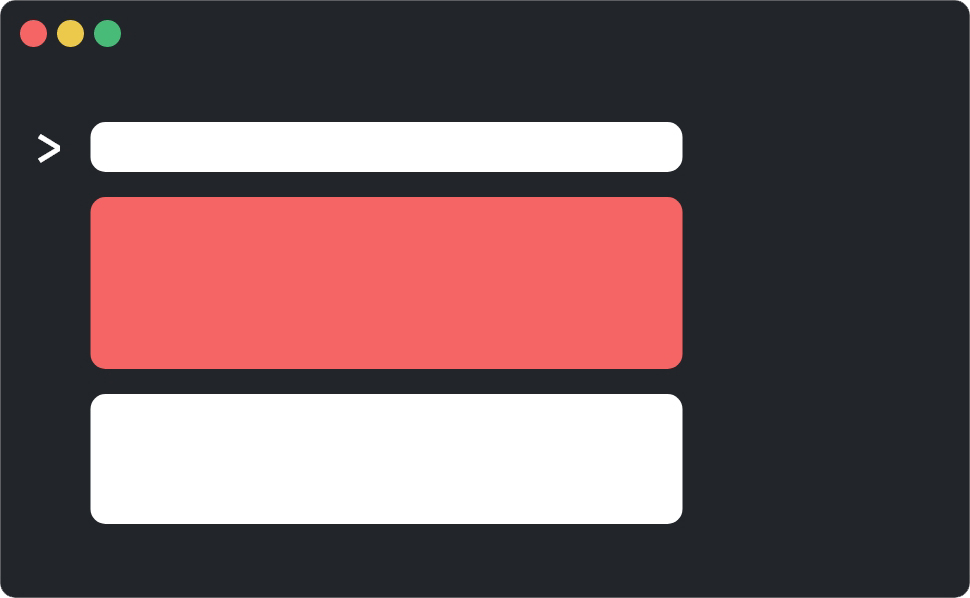
\includegraphics[width=0.4\textwidth]{errors}
    \caption{Error logging concept}
    \label{fig:nuua_errors}
\end{figure}

The first white line should include the \emph{absoltute} path of the source file followed by the line and the column where the error happened.

The red paragraph should include an error description of the error that caused the crash. This paragraph must have a fixed width to ensure
the error has a readable format.

The last white paragraph contains the line as seen in the source code of the program. The line must also include a reference to the column
where the error happened so that a quick look at the line can determine the problem.


\section{Logger entities}

The logger entity has all the properties that are mandatory fora log.
This includes the absolute file path of the source program, the line of the file where the error happened
and the column. Additionally, the error message that it has associated. A code representation is shown in
the \autoref{ls:logger_entity}.

\begin{listing}[H]
\begin{minted}{cpp}
// Represents a log entity.
class LoggerEntity {
    public:
        // Stores the file where the log comes from.
        const std::shared_ptr<const std::string> file;
        // Stores the line of the log.
        const line_t line;
        // Stores the column of the log.
        const column_t column;
        // Stores the message of the log.
        const std::string msg;
        // Creates a new log entity.
        LoggerEntity(
            const std::shared_ptr<const std::string> &file,
            const line_t line,
            const column_t column,
            const std::string &msg
        ) : file(file), line(line), column(column), msg(msg) {}
};
\end{minted}
\caption{Logger entity class}
\label{ls:logger_entity}
\end{listing}

\section{Logger class}

\autoref{ls:logger_class} shows a logger class implementation that satisfies all the previous statements.
In short, it stores a list of all the log entities and provides methods to add and remove logs. It also provides a crash
method that outputs the logs and returns an exit code without calling \texttt{exit()}.

\begin{listing}[H]
\begin{minted}{cpp}
// Represents the logger used in the whole toolchain.
class Logger
{
    // Stores all the log entities.
    std::vector<LoggerEntity> entities;
    // Displays a specific log entity.
    void display_log(const uint16_t index, const bool red) const;
    public:
        // Stores the executable path.
        std::string executable_path;
        // Adds a new entity to the entity stack.
        void add_entity(
            const std::shared_ptr<const std::string> &file,
            const line_t line,
            const column_t column,
            const std::string &msg
        );
        // Pops an entity from the entity stack.
        void pop_entity();
        // Crashes the program by displaying the entity stack
        // and further returning an apropiate exit code.
        int crash() const;
};
\end{minted}
\caption{Logger entity class}
\label{ls:logger_class}
\end{listing}

\section{Cross-platform caveat}

Due to the fact that Nuua is supported in multiple platforms, there is an important feature mentioned that must be
handled manually. The colored red output must be portable across all the major platforms. Windows is the platform that
is most special and therefore, special treatment must be taken.

For windows platforms, the C++ header \texttt{windows.h} must be included.
This header includes special functions to work with the windows terminal. The preprocessor macros
\texttt{\_WIN32} and \texttt{\_WIN64} can be used to determine if the windows header is needed.

Figure \autoref{ls:red_printf} shows the implementation of a red \texttt{printf} function working under all the major
platforms.

\begin{listing}[H]
\begin{minted}{cpp}
#if defined(_WIN32) || defined(_WIN64)
    #include <windows.h>
#endif
#include <stdio.h>
#include <stdarg.h>
#include <cstdlib>

static int red_printf(const char *format, ...)
{
    va_list arg;
    int result;
    va_start(arg, format);
    #if defined(_WIN32) || defined(_WIN64)
        HANDLE hConsole = GetStdHandle(STD_OUTPUT_HANDLE);
        CONSOLE_SCREEN_BUFFER_INFO consoleInfo;
        WORD saved_attributes;
        GetConsoleScreenBufferInfo(hConsole, &consoleInfo);
        saved_attributes = consoleInfo.wAttributes;
        SetConsoleTextAttribute(hConsole, FOREGROUND_RED);
        result = vfprintf(stderr, format, arg);
        SetConsoleTextAttribute(hConsole, saved_attributes);
    #else
        // \x1b[31m\x1b[0m = (9 + '\0')
        char *fmt = malloc(sizeof(char) * (strlen(format) + 10));
        strcpy(fmt, "\x1b[31m");
        strcat(fmt, format);
        strcat(fmt, "\x1b[0m");
        result = vfprintf(stderr, fmt, arg);
        free(fmt);
    #endif
    va_end(arg);
    return result;
}
\end{minted}
\caption{Red printf function}
\label{ls:red_printf}
\end{listing}


\chapter{Lexer}
The lexer is the lowest layer in the Nuua system as shown in \autoref{fig:nuua_system}. The lexer job is to transform
the program source code into a list of tokens. This step is also known as lexical analysis or tokenization.

\begin{figure}[H]
    \centering
    \begin{tikzpicture}
        [node distance=1cm]

        % Nodes of the layered system
        \node[block] (input) {List of characters};
        \node[block,right=of input] (lexer) {Lexer};
        \node[block,right=of lexer] (output) {List of tokens};

        % Lines
        \draw[line] (input) -- (lexer);
        \draw[line] (lexer) -- (output);

    \end{tikzpicture}

    % Caption and Label
    \caption{Lexer overview}
    \label{fig:lexer_overview}
\end{figure}

The lexer needs to provide an API to the layer above and one of the parameters of the scan function is the path of the
source file to scan. The lexer is also responsible for opening the file and creating a \texttt{char} array with its contents. This can be
done in the lexer class constructor seen in \autoref{ls:lexer_class}.
When the layer above wishes to scan the tokens the tokenization begins and therefore a list of tokens is built and returned.

\section{Strategy}

The strategy of the lexer is to use a state machine to determine the pattern of the tokens and be able to identify
what token type it's being scanned. The state machine finds a pattern and creates a specific token depending on
the state it landed. The state machine can also lead to no pattern. If there's a sequence of characters that don't match
a pattern, an error is then thrown using the logger module as described in \autoref{sec:logger}.

The implementation uses a C++ \texttt{switch} statement to match the first character of the pattern and further continues if needed
depending on the patterns.

In case a \texttt{\textbackslash n} is found, the lexer line is incremented and the column is reset to $0$. Since the current line and column
are properties in the lexer instance they only affect a single instance allowing multiple instances to scan different files at the same
time. \autoref{fig:finite_state_strings} shows an example pattern found in the lexer.

\begin{figure}[H]
	\centering
    \begin{subfigure}{\textwidth}
		\centering
        \begin{tikzpicture}[node distance=3cm]
            % Nodes
            \node[state] (1) {\texttt{S1}};
            \node[state, below left of=1] (2) {\texttt{S2}};
            \node[state, below right of=1] (3) {\texttt{S3}};
            % Lines
            \draw[line] (1) edge[left, bend right] node[xshift=-0.15cm, yshift=0.15cm] {\texttt{e1}} (2);
            \draw[line] (2) edge[loop left] node[xshift=-0.15cm] {\texttt{e2}} (2);
            \draw[line] (2) edge[below, bend right] node[yshift=-0.15cm] {\texttt{e3}} (3);
            \draw[line] (3) edge[right, bend right] node[xshift=0.15cm, yshift=0.15cm] {\texttt{e4}} (1);
        \end{tikzpicture}
		\caption{Diagram}
	\end{subfigure}
	\begin{subtable}{0.45\textwidth}
		\centering
        \begin{tabular}{ l p{4.5cm} }
            \textbf{State} & \textbf{Explanation} \\
            \texttt{S1} & Initial state of the state machine. \\
            \texttt{S2} & Build string. \texttt{s += c} \\
            \texttt{S3} & Create token \\
		\end{tabular}
		\caption{State table}
	\end{subtable}
	\begin{subtable}{0.45\textwidth}
		\centering
        \begin{tabular}{ l l l }
            \textbf{Event} & \textbf{Condition} & \textbf{Action} \\
            \texttt{e1} & \texttt{c == '"'} & \texttt{c = next\_char()} \\
            \texttt{e2} & \texttt{c != '"'} & \texttt{c = next\_char()} \\
            \texttt{e3} & \texttt{c == '"'} & \texttt{-} \\
            \texttt{e4} & \texttt{-} & \texttt{c = next\_char()} \\
		\end{tabular}
		\caption{Event table}
	\end{subtable}
	\caption{Example finite state machine for strings}
    \label{fig:finite_state_strings}
\end{figure}

As shown in \autoref{fig:scanner}, an efficient way to scan the file is using two pointers to some of the \texttt{chars} found in the source file.
The first pointer points to the start of the token being scanned and the second one advances accordingly with the help of the
state machine. When the state machine determines that a new token must be created the start pointer is used as the first character
pointer in the token as explained in \autoref{sec:tokens} and the length of the token can be determined by using pointer arithmetic given:

\begin{center}
$\texttt{length} = \texttt{current\_ptr} - \texttt{start\_ptr} + 1$
\end{center}

Since the string values can ignore the two \texttt{'"'} found at the
start and at the end of the token, the length will be decremented by two and the start pointer is incremented by one to get only the string value.
When a blank space is found in the initial state of the state machine the \texttt{start\_ptr} pointer address is then set to the \texttt{current\_ptr} address
and the current parser column increases.

\begin{figure}[H]
    \centering
    \begin{tikzpicture}[node distance=1cm]
        % Nodes
        \node[square, minimum height=0.75cm, minimum width=1cm,] (n1) {...};
        \node[square, minimum height=0.75cm, minimum width=1cm, right of=n1] (n2) {\texttt{"}};
        \node[square, minimum height=0.75cm, minimum width=1cm, right of=n2] (n3) {\texttt{a}};
        \node[square, minimum height=0.75cm, minimum width=1cm, right of=n3] (n4) {\texttt{b}};
        \node[square, minimum height=0.75cm, minimum width=1cm, right of=n4] (n5) {\texttt{c}};
        \node[square, minimum height=0.75cm, minimum width=1cm, right of=n5] (n6) {\texttt{"}};
        \node[square, minimum height=0.75cm, minimum width=1cm, right of=n6] (n7) {...};
        % Lines
        \draw[line] ($(n2.south) + (0, -0.75)$) node[anchor=north] {\texttt{start\_ptr}} -- (n2);
        \draw[line] ($(n6.south) + (0, -0.75)$) node[anchor=north] {\texttt{current\_ptr}} -- (n6);
    \end{tikzpicture}
    \caption{Lexer scan technique}
    \label{fig:scanner}
\end{figure}

\section{Tokens}
\label{sec:tokens}

Tokens represent specific lexeme patterns. The list of the patterns and the tokens associated with it can be seen on \autoref{fig:nuua_tokens_1},
\autoref{fig:nuua_tokens_2} and \autoref{fig:nuua_tokens_3}. The tokens must also take into consideration escaping characters. For example, a string
representation might be willing to use the char \texttt{'"'} as part of the string value and not determine the end of the string. Therefore, there
is a list of escaped chars that are taken into consideration as shown in \autoref{sec:espaced_chars}.

\begin{table}[H]
	\centering
	\begin{subtable}{0.45\textwidth}
		\centering
        \begin{tabular}{ l l }
            \textbf{Pattern} & \textbf{Token} \\
            \texttt{\textbackslash n} & \texttt{TOKEN\_NEW\_LINE} \\
            \texttt{(} & \texttt{TOKEN\_LEFT\_PAREN} \\
            \texttt{)} & \texttt{TOKEN\_RIGHT\_PAREN} \\
            \texttt{\{} & \texttt{TOKEN\_LEFT\_BRACE} \\
            \texttt{\}} & \texttt{TOKEN\_RIGHT\_BRACE} \\
            \texttt{,} & \texttt{TOKEN\_COMMA} \\
            \texttt{.} & \texttt{TOKEN\_DOT} \\
            \texttt{..} & \texttt{TOKEN\_DOUBLE\_DOT} \\
            \texttt{...} & \texttt{TOKEN\_TRIPLE\_DOT} \\
            \texttt{-} & \texttt{TOKEN\_MINUS} \\
		\end{tabular}
		\caption{}
	\end{subtable}
	\begin{subtable}{0.45\textwidth}
		\centering
        \begin{tabular}{ l l }
            \textbf{Pattern} & \textbf{Token} \\
            \texttt{+} & \texttt{TOKEN\_PLUS} \\
            \texttt{/} & \texttt{TOKEN\_SLASH} \\
            \texttt{*} & \texttt{TOKEN\_STAR} \\
            \texttt{->} & \texttt{TOKEN\_RIGHT\_ARROW} \\
            \texttt{!} & \texttt{TOKEN\_BANG} \\
            \texttt{!=} & \texttt{TOKEN\_BANG\_EQUAL} \\
            \texttt{=} & \texttt{TOKEN\_EQUAL} \\
            \texttt{==} & \texttt{TOKEN\_EQUAL\_EQUAL} \\
            \texttt{>} & \texttt{TOKEN\_HIGHER} \\
            \texttt{>=} & \texttt{TOKEN\_HIGHER\_EQUAL} \\
		\end{tabular}
		\caption{}
	\end{subtable}
	\caption{Nuua tokens (1)}
    \label{fig:nuua_tokens_1}
\end{table}

\begin{table}[H]
	\centering
	\begin{subtable}{0.45\textwidth}
		\centering
        \begin{tabular}{ l l }
            \textbf{Pattern} & \textbf{Token} \\
            \texttt{=>} & \texttt{TOKEN\_BIG\_RIGHT\_ARROW} \\
            \texttt{:} & \texttt{TOKEN\_COLON} \\
            \texttt{return} & \texttt{TOKEN\_RETURN} \\
            \texttt{print} & \texttt{TOKEN\_PRINT} \\
		\end{tabular}
		\caption{}
	\end{subtable}
	\begin{subtable}{0.45\textwidth}
		\centering
        \begin{tabular}{ l l }
            \textbf{Pattern} & \textbf{Token} \\
            \texttt{use} & \texttt{TOKEN\_USE} \\
            \texttt{from} & \texttt{TOKEN\_FROM} \\
            \texttt{elif} & \texttt{TOKEN\_ELIF} \\
            \texttt{in} & \texttt{TOKEN\_IN} \\
            \texttt{export} & \texttt{TOKEN\_EXPORT} \\
		\end{tabular}
		\caption{}
	\end{subtable}
	\caption{Nuua tokens (2)}
    \label{fig:nuua_tokens_2}
\end{table}

\begin{table}[H]
	\centering
	\begin{subtable}{0.45\textwidth}
		\centering
        \begin{tabular}{ l l }
            \textbf{Pattern} & \textbf{Token} \\
            \texttt{<} & \texttt{TOKEN\_LOWER} \\
            \texttt{<=} & \texttt{TOKEN\_LOWER\_EQUAL} \\
            \texttt{<IDENTIFIER>} & \texttt{TOKEN\_IDENTIFIER} \\
            \texttt{<STRING\_EXPR>} & \texttt{TOKEN\_STRING} \\
            \texttt{<INTEGER\_EXPR>} & \texttt{TOKEN\_INTEGER} \\
            \texttt{<FLOAT\_EXPR>} & \texttt{TOKEN\_FLOAT} \\
            \texttt{as} & \texttt{TOKEN\_AS} \\
            \texttt{or} & \texttt{TOKEN\_OR} \\
            \texttt{and} & \texttt{TOKEN\_AND} \\
            \texttt{class} & \texttt{TOKEN\_CLASS} \\
		\end{tabular}
		\caption{}
	\end{subtable}
	\begin{subtable}{0.45\textwidth}
		\centering
        \begin{tabular}{ l l }
            \textbf{Pattern} & \textbf{Token} \\
            \texttt{fun} & \texttt{TOKEN\_FUN} \\
            \texttt{else} & \texttt{TOKEN\_ELSE} \\
            \texttt{true} & \texttt{TOKEN\_TRUE} \\
            \texttt{false} & \texttt{TOKEN\_FALSE} \\
            \texttt{while} & \texttt{TOKEN\_WHILE} \\
            \texttt{for} & \texttt{TOKEN\_FOR} \\
            \texttt{if} & \texttt{TOKEN\_IF} \\
            \texttt{\textbackslash 0} & \texttt{TOKEN\_EOF} \\
            \texttt{[} & \texttt{TOKEN\_LEFT\_SQUARE} \\
            \texttt{]} & \texttt{TOKEN\_RIGHT\_SQUARE} \\
		\end{tabular}
		\caption{}
	\end{subtable}
	\caption{Nuua tokens (3)}
    \label{fig:nuua_tokens_3}
\end{table}

To make an efficient token representation, instead of copying the \texttt{char} array (lexeme) that matches that token pattern
a reference to the first character of the token is saved into the token instance and then the length is specified to know how many
chars it does consist of. That way, no unnecessary memory is added to each token. The only needed thing is to keep the source code \texttt{char}
array in memory and avoid reallocations till the token instance is not needed anymore. \autoref{fig:scanner_token} shows a visual representation.
\autoref{ls:token_class} shows the token representation that is used in the Nuua compiler.

Among other information, the type of the token (as shown in \autoref{fig:nuua_tokens_1}, \autoref{fig:nuua_tokens_2} and \autoref{fig:nuua_tokens_3})
is also stored as part of the token. Additionally, the line and column where that token was found is also stored.\\

\begin{figure}[H]
    \centering
    \begin{tikzpicture}[node distance=1cm]
        % Nodes
        \node[square, minimum height=0.75cm, minimum width=1cm] (n0) {Source code};
        \node[square, minimum height=0.75cm, minimum width=1cm, right = -0.025cm of n0.east] (n1) {...};
        \node[square, minimum height=0.75cm, minimum width=1cm, right of=n1] (n2) {\texttt{w}};
        \node[square, minimum height=0.75cm, minimum width=1cm, right of=n2] (n3) {\texttt{h}};
        \node[square, minimum height=0.75cm, minimum width=1cm, right of=n3] (n4) {\texttt{i}};
        \node[square, minimum height=0.75cm, minimum width=1cm, right of=n4] (n5) {\texttt{l}};
        \node[square, minimum height=0.75cm, minimum width=1cm, right of=n5] (n6) {\texttt{e}};
        \node[square, minimum height=0.75cm, minimum width=1cm, right of=n6] (n7) {...};
        % Token nodes
        \node[square, anchor=west, minimum height=0.75cm] at ($(n0.south west) + (0, -2)$) (token) {Token Instance};
        \node[square, minimum height=0.75cm, right = -0.025cm of token.east] (token1) {\texttt{const char *start = \phantom{X}}};
        \node[square, minimum height=0.75cm, right = -0.025cm of token1.east] (token2) {\texttt{const uint32\_t length = 5}};
        % Lines
        \draw[dot_arrow] ($(token1.east) + (-0.2, -0.05)$) -- (n2.south);
    \end{tikzpicture}
    \caption{Lexer token technique}
    \label{fig:scanner_token}
\end{figure}

\begin{listing}[H]
\begin{minted}{cpp}
class Token
{
    public:
        // The type of the token.
        const TokenType type;
        // A pointer to the first char.
        // (Not used as a null terminated char array)
        const char *start;
        // The length of the token.
        const uint32_t length;
        // The line where it is found.
        const line_t line;
        // The column where it is found.
        const column_t column;
        // String representation of the token names.
        static std::vector<std::string> token_names;
        // Pattern matching a token name.
        static std::vector<std::string> type_names;
        // Contains the escaped chars of the language.
        static const std::unordered_map<char, char> escaped_chars;
        // Create a new instance of a token given the
        // required parameters.
        Token(
            const TokenType type,
            const char *start,
            const uint32_t length,
            const line_t line,
            const column_t column
        ) : type(type), start(start), length(length),
            line(line), column(column) {}
        // Debug the token by printing it on the
        // screen with the correct format.
        void debug_token() const;
        // Convert the token to a string representation.
        std::string to_string() const;
        // Convert the token to its pattern string representation.
        std::string to_type_string() const;
};
\end{minted}
\caption{Token class}
\label{ls:token_class}
\end{listing}

\section{Lexer Class}

The lexer class represents a lexer instance to scan a file and return a list of tokens.
\autoref{ls:lexer_class} shows the code used in the Nuua compiler to transform a \texttt{char} array
corresponding to the source file to a list of token instances.

\begin{listing}[H]
\begin{minted}{cpp}
class Lexer
{
    // Stores the file where the tokens are being scanned.
    std::shared_ptr<const std::string> file;
    // Stores the start char of the token being scanned.
    const char *start;
    // Stores the current char of the token beeing scanned.
    const char *current;
    // Stores the current line in the source file.
    line_t line;
    // Stores the current column in the source file.
    column_t column;
    // Stores a list of reserved words for the identifiers.
    static const std::unordered_map<std::string, TokenType> reserved_words;
    // Generates a token error.
    const std::string token_error() const;
    // Build the token and set the start char to the current one.
    Token make_token(TokenType type);
    // Helper to build tokens.
    bool match(const char c);
    TokenType is_string(bool simple);
    TokenType is_number();
    TokenType is_identifier();
    // Reads a file and stores the contents in the current instance.
    void read_from_file(const std::shared_ptr<const std::string> &file);
    public:
        // Stores the source code of the file.
        std::unique_ptr<std::string> source;
        // Scans the source and stores the tokens.
        void scan(std::unique_ptr<std::vector<Token>> &tokens);
        // Initializes a lexer given a file name.
        Lexer(const std::shared_ptr<const std::string> &file);
};
\end{minted}
\caption{Lexer class}
\label{ls:lexer_class}
\end{listing}


\chapter{Parser}
The job of the parser is to transform the list of tokens returned by the Lexer into an abstract syntax tree.\\

\begin{figure}[H]
    \centering
    \begin{tikzpicture}
        [node distance=1cm]

        % Nodes of the layered system
        \node[block] (input) {List of tokens};
        \node[block,right=of input] (parser) {Parser};
        \node[block,right=of lexer] (output) {Abstract Syntax Tree};

        % Lines
        \draw[line] (input) -- (parser);
        \draw[line] (parser) -- (output);

    \end{tikzpicture}

    % Caption and Label
    \caption{Parser overview}
    \label{fig:parser_overview}
\end{figure}

There are a lot of different algorithms and strategies for parsing different set of grammars.
There are also a lot of parser generators out there that can help building a parser. However, this thesis implements
a hand written top down recursive descend predictive parser for the following main reasons:

\begin{enumerate}
    \item To have as much control as needed over the parser. Specially for error reporting.
    \item To enforce a zero-policy rule.
    \item Easy to build and fast enough for the job.
    \item To learn how to build a recursive descend parser and learn how it works.
\end{enumerate}

Recursive descend parsers are probably the simplest way to build a parser as mentioned in \autocite[Section~6]{crafting_interpreters}.
In fact, even if it's a simple parser it's used in very famous and large projects like \texttt{GCC} or \texttt{V8}.

As can be seen on \autocite{top_down_parsing} the top down parers can be classified into the ones using backtracking and the ones using a predictive technique.

\begin{itemize}
    \item \emph{Backtracking parsers}: Backtracking parsers try to guess the correct production rule based on the current token. This guess can however, lead to a
        dead-end and therefore a backtrack is needed to go back and make anothe decision. This is hoever, very inefficient for programming languages due the ammount
        of nonterminals found in them.
    \item \emph{Predictive parsers}: Predictive parsers choose the production rule acording to the current token and the next token found. The next tooken is called
        a lookahead token. Predictive parsers have a major issue with left-recursion and therefore, the language grammar needs to be adapted to it.
        The Nuua grammar as seen on \autoref{sec:nuua_grammar} is already adapted for left-recursion based on the solution mentioned on
        \autocite[Section~6]{crafting_interpreters}.
\end{itemize}

A recursive descend parser is a possible technique for implementing a top-down predictive parser that consists in the creation of a funciton for each
nonterminal found in the grammar and then calling the functions depending on the current token and the lookahead.

\section{Abstract Syntax Tree}

\section{Block Scope}

\section{Data Types}

\section{Tree Nodes}

\section{Parser Class}


\chapter{Semantic Analyzer}
\label{sec:semantic_analysis}
The semantic analyzer is ran after the AST has been generated and therefore the program is all in
the same data structure. The job of the semantic analyzer is not to transform the AST but to analyze it.
There is the possibility for optimizations to be performed during the analysis to improve the resulting code.
This includes for instance loop unrolling, constant folding or dead code elimination. However, those things
are not part of this thesis and therefore those optimizations have been mentioned in \autoref{sec:forthcoming}.
However, this thesis deals with other types of optimizations. Specifically, bytecode optimization is performed to some extend.

In short, the job of the analyzer is to perform the following things:

\begin{itemize}
    \item Create the symbol table for each scope and block found. This include all module scopes and each block scope found.
    \item Get all the type information from the expressions.
    \item Perform the semantic checks on all the statements and expressions found in the AST. All the requirements for those nodes
        are explained in \autoref{sec:statements} and \autoref{sec:expressions} respectively.
    \item Add specific node information. This information has been mentioned individually on each tree node on \autoref{sec:tree_nodes}.
\end{itemize}

\section{Technique}

Before any analysis begins, a full module scope analysis needs to be performed. This is done to ensure that when functions are analyzed
(and so do their statements) the module scope is already valid and contains the information needed to have a correct statement analysis. For instance
if a function have a statement that makes a call to another function on the module, that callee function must be known, so its signature needs to be
analyzed before.

To solve this, a first analysis is performed only on the top level declarations (module scope) found in the module.
If one of the top level declarations is a use declaration, then that module is first analyzed completly while the current one waits.
The top level analysis just gets information about the top level declarations and does not perform further analysis.
That means that it just gets the information of the functions, classes and so on without analyzing the function bodies.
Top level classes are also analyzed only on the top level of their bodies. Once all this phase is complete, the code analysis begin in an arbitrary order.
This can be done as the top level is already analyzed and therefore all the symbol table for the module block is already built and the types are known.

Once the code analysis begin the function bodies are analyzed and so do classes methods. The analysis run by recursively walking the AST and further performing
all the checks mentioned in \autoref{sec:statements} and on \autoref{sec:expressions} depending on the type of node beeing analyzed.
This analysis is also recursive.

\begin{figure}[H]
	\centering
	\begin{subtable}{0.45\textwidth}
        \texttt{fun main(argv: [string]) \{\\\tab// ...\\\}}
		\caption{Program}
	\end{subtable}
	\begin{subtable}{0.45\textwidth}
		\centering
        \texttt{
            TOKEN\_FUN TOKEN\_IDENTIFIER TOKEN\_LEFT\_PAREN TOKEN\_IDENTIFIER TOKEN\_COLON TOKEN\_LEFT\_SQUARE TOKEN\_IDENTIFIER
            TOKEN\_RIGHT\_SQUARE TOKEN\_RIGHT\_PAREN TOKEN\_LEFT\_BRACE TOKEN\_NEW\_LINE
            TOKEN\_RIGHT\_BRACE TOKEN\_NEW\_LINE
            TOKEN\_EOF
        }
		\caption{List of tokens}
	\end{subtable}
    \begin{subfigure}{0.45\textwidth}
		\centering
        \begin{tikzpicture}[node distance=1.75cm]
            % Nodes
            \node[state] (0) {\texttt{P(1)}};
            \node[state, below of=0] (1) {\texttt{F1}};
            \node[state, below left of=1] (3) {\texttt{P2}};
            \node[state, left of=3] (2) {\texttt{P1}};
            \node[state, below right of=1] (4) {\texttt{P3}};
            \node[state, right of=4] (5) {\texttt{P4}};
            \node[state, below of=5] (6) {\texttt{...}};
            % Legend
            \node[text width=4.5cm, align=left, right = 0.5cm of 0.east] (l) {

                { \footnotesize \noindent
                    \texttt{F1: function}\\
                    \texttt{P1: name:\\\quad main}\\
                    \texttt{P2: parameters\\\quad argv: [string]}\\
                    \texttt{P3: return\_type\\\quad no\_value}\\
                    \texttt{P4: body}
                }
            };
            % Lines
            \draw (0) -- (1);
            \draw (1) -- (2);
            \draw (1) -- (3);
            \draw (1) -- (4);
            \draw (1) -- (5);
            \draw (5) -- (6);
        \end{tikzpicture}
		\caption{Abstract Syntax Tree}
	\end{subfigure}
    \begin{subfigure}{0.45\textwidth}
		\centering
        \begin{tabular}{ l l l }
            \textbf{Variable} & \textbf{Type} \\
            \texttt{main} & \texttt{([string])} \\
		\end{tabular}
		\caption{Module scope symbol table}
	\end{subfigure}
	\caption{Example program top level analysis}
    \label{fig:ast_example}
\end{figure}

Among other mentioned checks that are specific to certain nodes, some of the checks the analyzer performs are:

\begin{itemize}
    \item Declared variables.
    \item Function return value match.
    \item Functions without return type usage.
    \item Argument type match.
    \item Assignment type match.
    \item List / String / Dictionary index type.
    \item Variable lifetime (\texttt{last\_use}).
    \item Use only exported declarations.
    \item Check for iterator (must be list / dict).
    \item Type matching.
    \item \texttt{main([string])} required on the main module.
\end{itemize}

\section{Module class}

The module class is used to analyze a module. It automatically creates a new instance of it when it needs to analyze
the AST of a use declaration.\\

\begin{code}
\begin{minted}{cpp}
class Module
{
    // Stores the file name of that module.
    std::shared_ptr<const std::string> file;
    // Stores the code of that module.
    std::shared_ptr<std::vector<std::shared_ptr<Statement>>> code;
    // Stores the blocks used while analyzing the module.
    std::vector<std::shared_ptr<Block>> blocks;
    // Return variable if needs to be checked. Only 1 can exist since
    // it can only analyze 1 function at a time.
    std::shared_ptr<Type> return_type;
    // Analyzes the TLDs of the current module.
    void analyze_tld();
    // Analyzes the given top level declaration.
    void analyze_tld(const std::shared_ptr<Statement> &tld, const bool set_exported = false);
    // Analyzes the class top level declarations.
    // void analyze_class_tld(const std::shared_ptr<Class> &c);
    void analyze_class_tld(const std::shared_ptr<Statement> &tld, const std::shared_ptr<Block> &block);
    // Analyzes the code.
    void analyze_code();
    // Analyzes the statement.
    void analyze_code(const std::shared_ptr<Statement> &rule, bool no_declare = false);
    // Analyzes the expression.
    void analyze_code(const std::shared_ptr<Expression> &rule, const bool allowed_noreturn_call = false);
    // Analyzes the block.
    std::shared_ptr<Block> analyze_code(
        const std::vector<std::shared_ptr<Statement>> &code,
        const std::vector<std::shared_ptr<Declaration>> &initializers = std::vector<std::shared_ptr<Declaration>>(),
        const std::shared_ptr<Node> &initializer_node = std::shared_ptr<Node>()
    );
    // Declares a variable to the most top level block.
    void declare(const std::shared_ptr<Declaration> &dec, const std::shared_ptr<Node> &node = std::shared_ptr<Node>());
    // Check if the given module have all the classes defined.
    bool check_classes(const std::vector<std::string> &classes, const std::shared_ptr<Node> &fail_at);
    public:
        // Stores the main block of that module.
        std::shared_ptr<Block> main_block = std::make_shared<Block>();
        // Main module constructor
        Module(std::shared_ptr<const std::string> &file)
            : file(file) {}
        // Analyzes the module and adds it's entry to the modules symbol table.
        std::shared_ptr<Block> analyze(std::shared_ptr<std::vector<std::shared_ptr<Statement>>> &code, const bool require_main = false);
};
\end{minted}
\end{code}

\section{Module In-memory Cache}

Since a module might be imported more than once as shown in \autoref{fig:module_mem_cache} the analyzer
have an in-memory cache to know when a module has been analyzed to avoid redundant analyses.
Once a module has been analyzed it is added into a list of analyzed modules and when a new module is required to be
analyzed is first checked if it has been. If so, it returns its module scope symbol table.


\chapter{Code generator}
The code generation layer is responsible for generating the bytecode that will be interpreted by the virtual machine.
Bytecode instructions are very similar to hardware instructions but at a much higher level (they are not as close to hardware).
\autoref{fig:codegen_overview} shows the job of the code generator.

This chapter does not define all the available opcodes found in Nuua. All those opcodes can be found on \autoref{sec:opcodes}.

\begin{figure}[H]
    \centering
    \begin{tikzpicture}
        [node distance=1cm]

        % Nodes of the layered system
        \node[block] (input) {Abstract syntax tree};
        \node[block,right=of input] (codegen) {Code generator};
        \node[block,right=of lexer] (output) {List of opcodes};

        % Lines
        \draw[line] (input) -- (codegen);
        \draw[line] (codegen) -- (output);

    \end{tikzpicture}

    % Caption and Label
    \caption{Code generator overview}
    \label{fig:codegen_overview}
\end{figure}

The goal of this layer is to be able to transform a data structure into a linear sequence of opcodes. The opcodes have been designed
for the needs of the project. This transformation is performed in a similar way as the semantic analysis explained in \autoref{sec:semantic_analysis}.
It first performs a top-level walk to assign each function a register (known as tld registration) and if a use declaration is found, it is also
registered by after the current module. Therefore, it delays it's registration until the current one it's analyzed. This has no impact on the resulting code
rather than having each module registered sequentially (easier to debug).

\section{Call Stack and Frames}
\label{sec:call_stack}

Each function call in Nuua introduces a new frame that is pushed into the call stack. The call stack is a stack that stores the active frames in the application.
When the function ends the frame is popped from the call stack. The frame contains information about the function variables, specifically, it contains the registers
where the function values live. Space is allocated when the frame is created and it's then deallocated when the function ends. This is done by the
virtual machine as seen in \autoref{sec:virtual_machine}.

The frame consists of an array containing the registers that the function use. Those registers are allocated when the frame is created (when a function is called).
They must also contain the amount of registers it has allocated and a return address that is used by the virtual machine to go back to the opcode where the function was called.

To allow passing parameters between frames (function parameters and return values) all frames share a common value stack. When a function is called, its arguments
are pushed to the stack and once the function frame is set they are poped from it. When a function returns a value, it is pushed to the stack and the frame ends.
When the last frame is restored, it then pops the value to a register for further use.

Therefore, \autoref{ls:frame_class} shows the frame class that is used in the Nuua compiler and virtual machine.

\begin{listing}[H]
\begin{minted}{cpp}
class Frame
{
    public:
        // Stores the registers.
        std::unique_ptr<Value[]> registers;
        // Stores the registers size.
        registers_size_t registers_size = 0;
        // Stores the return address to get back to the original program counter.
        opcode_t *return_address = nullptr;
        // Allocates the space to store the registers.
        void allocate_registers(registers_size_t size);
        // Frees the allocated register space.
        void free_registers();
        // Setup the frame.
        void setup(registers_size_t size, opcode_t *return_address);
};
\end{minted}
\caption{Frame class}
\label{ls:frame_class}
\end{listing}

\section{Register Allocation}

Compiler allocation takes place during code generation by the use of a \texttt{FrameInfo} class that helps to determine the right amount of registers needed
to compile a function and also optimizes the registers used by using a very simple strategy. The frame information class is shown in \autoref{ls:frame_info_class}.

As it can be seen, the frame info is used as a register allocator, it basically consists of two lists of registers and a current register index.

\begin{itemize}
    \item \emph{Free Registers}: Stores the registers that were freed and can be used again.
    \item \emph{Protected Registers}: Stores the registers that are protected from being freed (as they are used in variables and not anonymous expressions).
    \item \emph{Current Register}: Stores the index of the register that will be given in case no free register is available.
\end{itemize}

\begin{listing}[H]
\begin{minted}{cpp}
class FrameInfo
{
    // Stores the registers that are free to use again.
    std::vector<register_t> free_registers;
    // Stores the registers that are protected to get free unless forçed.
    std::vector<register_t> protected_registers;
    public:
        // Stores the next register to give in case no free ones are available.
        register_t current_register = 0;
        // Method to return an available register.
        // It will try to get it from the free_registers
        // otherwise it will return a new register and
        // increment current_register by 1
        register_t get_register(bool protect = false);
        // Used to free a register.
        void free_register(register_t reg, bool force = false);
        // Resets the frame info.
        void reset();
};
\end{minted}
\caption{FrameInfo class}
\label{ls:frame_info_class}
\end{listing}

When the function \texttt{get\_register} is called, it first performs a check on the \texttt{free\_registers} list. If that list is empty it means
that there is no free register to be used, and therefore the \texttt{current\_register} index is the register that will be given and it's incremented by 1.
If the list is not empty it means that there are free registers available and then the last element of the list is poped and is the register that will be given.
In any case, if the \texttt{protect} parameter is true the given register is also added to the \texttt{protected\_registers} list before the function ends.

When the function \texttt{free\_register} is called, it first performs a check to see if the register that is attempted to be freed is a protected register.
If it is protected and the \texttt{force} parameter is false the function ends without any modifications. If it is protected and the \texttt{force} parameter
is true, the element it's removed from the \texttt{protected\_registers} and the register is added to the \texttt{free\_registers} list. In case the register
it's not in the \texttt{protected\_registers} list, it is added to the \texttt{free\_registers} list without any further checks.

The reason behind this strategy is because when the code generation is taking place each node in the AST gets compiled and simple expressions like
\texttt{1 + 2} need to use 3 registers. 1 for the destination where the result of the operations is going to be stored (this calls the \texttt{get\_register}
function found in the register allocator) and 2 for the operands. However, when the operation is complete and the result is in the destination register,
the other 2 registers are not used again. They are then considered garbage. However, that means that not only they are garbage but they are also using
part of the memory that could be used by further registers.

The solution is to use the register allocator presented in \autoref{ls:frame_info_class} to free the values of the 2 registers
that can become garbage after the operation is complete. The reason there are protected registers is in case the operation was something
like \texttt{a + 2}. Where the register where the variable \texttt{a} is stored should not be freed because the variable could be used afterward.
This also means that when a variable is declared, the register that is bound to be a protected register and can only be freed when the
variable reaches the last node where it is used (This is already known since the semantic analysis determines the variable lifetime).
The variable can be freed by using the force parameter.

In the \autoref{fig:bytecode_rel} there can be seen that the registers where the same destination register is used in different operations. This is
thanks to this register allocation technique. The number of required registers for the function is also much lower needing much less space to allocate
in order to do all of its tasks.

\section{Program Memory}

The program memory represents the place where the program is going to be stored. Not only does include all the generated bytecode but also
includes the constant pool where all the constants are stored and also a way to store the relation between opcodes and their file, line, and column where
they are found in the program source file in case the virtual machine needs to throw an error.
The strategy used is explained in \autoref{sec:bytecode_origin}. \autoref{ls:memory_class} shows the class used in Nuua to represent the program memory.

\begin{listing}[H]
\begin{minted}{cpp}
class Memory
{
    public:
        // This stores the opcodes and consant indexes of the code.
        std::vector<opcode_t> code;
        // Stores the value constants.
        std::vector<Value> constants;
        // Stores the lines corresponding to the opcodes.
        std::unordered_map<size_t, std::shared_ptr<const std::string>> files;
        // Stores the lines corresponding to the opcodes.
        std::unordered_map<size_t, line_t> lines;
        // Stores the lines corresponding to the opcodes.
        std::unordered_map<size_t, column_t> columns;
        // Dumps the memory.
        void dump();
};
\end{minted}
\caption{Memory class}
\label{ls:memory_class}
\end{listing}

\subsection{Bytecode and Source File Relationship}
\label{sec:bytecode_origin}

The number of opcodes generated can be pretty high but it's not an issue considering each opcode is just $64$ bits (64 bits * operand).
However, each opcode should be bound to a file pointer, a line, and a column. This includes so many extra bytes for no reason. This would, however, be quite
easy to implement by creating 3 additional arrays with the same length of the opcodes + operands (again it uses a lot of memory). A proposed solution uses 3
hashmaps (for the files, lines, and columns) where the hashmap keys correspond to an arbitrary index in the bytecode array where the corresponding
value has changed.

This is better explained with an example as shown in \autoref{fig:bytecode_rel}. As the annotations on the right side of the bytecode show, there are only 3 line changes. Therefore, the hashmap that corresponds to the lines will have 3 entries where the keys are
the indexes where this line change occur. Following the same code we can deduce:

\begin{itemize}
    \item The first index is 0 with the value of 1.
    \item The second index 2 with the value of 2.
    \item The third index 19 with the value of 3.
\end{itemize}

This strategy allows deducing the line where the code failed by looking at the hashmap keys and getting
the value of the highest key that is lower or equal to the current index. Let's assume the code fails at the annotation marked with a \texttt{*}.
The fail index is 8 (the opcode is on index 8). By looking at the hashmap keys previously stated, the highest key lower than 8 is the key 2
and therefore the value is line 2.

The same strategy applies to the file and the column as well.

In short then, one of the jobs of the code generator is to add the necessary keys and values to the hashmaps.

\begin{figure}[H]
	\centering
	\begin{subtable}{0.4\textwidth}
\begin{minted}{cpp}
fun main(argv: [string]) {
    1 + 2 + 3
    4 + 5 + 6
}
\end{minted}
		\caption{Program}
	\end{subtable}
	\begin{subtable}{0.5\textwidth}
\begin{lstlisting}
POP     R-00000 // Line 1
LOAD_C  R-00001 C-00000 // Line 2
LOAD_C  R-00002 C-00001
ADD_INT R-00003 R-00001 R-00002 // *
LOAD_C  R-00002 C-00002
ADD_INT R-00001 R-00003 R-00002
LOAD_C  R-00002 C-00003 // Line 3
LOAD_C  R-00003 C-00004
ADD_INT R-00004 R-00002 R-00003
LOAD_C  R-00003 C-00005
ADD_INT R-00002 R-00004 R-00003
RETURN
EXIT
\end{lstlisting}
		\caption{Bytecode generated}
        \label{fig:bytecode_rel_bg}
	\end{subtable}
	\caption{Example program bytecode}
    \label{fig:bytecode_rel}
\end{figure}

\section{Program}

With the program memory taking care of all the opcodes, constants and the bytecode relationship with the source file, a program can be represented
by its memory and the main frame (where the global registers live).
\autoref{ls:program_class} shows the program class used in Nuua.

\begin{listing}[H]
\begin{minted}{cpp}
class Program
{
    public:
        // Stores the main frame of the program.
        Frame main_frame;
        // Stores the program memory (The main code).
        std::unique_ptr<Memory> memory;
        // Constructor to allocate the memory of the
        // program memory. Can't be done here since
        // Memory is a forward declared class.
        Program();
};
\end{minted}
\caption{Program class}
\label{ls:program_class}
\end{listing}

\section{Values}

Values are very important for the virtual machine, but the code generator is the one that defines how values look like since the code generator
already creates values (the constants) for the program. Therefore, the values need to be explained here. As \autoref{sec:nuua_data_types} explains, the
values may have any of those types but not more than one at the same time. The code generator defines the C++ data types for each value as
shown in \autoref{ls:type_defs}.

\begin{listing}[H]
\begin{minted}{cpp}
typedef int64_t nint_t;
typedef double nfloat_t;
typedef bool nbool_t;
typedef std::string nstring_t;
typedef std::vector<Value> nlist_t;
typedef ValueDictionary ndict_t;
typedef ValueFunction nfun_t;
typedef ValueObject nobject_t;
\end{minted}
\caption{Nuua data type definitions}
\label{ls:type_defs}
\end{listing}

A value must know its type and its current value. Due to the fact that the values are very different types but only a single one can exist at the same time, a
C union can be used to avoid wasting memory. Modern C++ has a \texttt{std::variant} that is basically a C union with steroids since it calls the
deconstructors when the data changes and also stores the type it owns. A value should be able to be retyped and changed without the need to
allocate a new value and deallocate an old one. Reusing memory is something that will be needed since registers are re-used and the fewer memory allocations,
the faster the execution becomes.

\begin{listing}[H]
\begin{minted}{cpp}
class Value
{
    void build_from_type(const Type *type);
    public:
        // The type of the value.
        Type type;
        // Using a variant to avoid unessesary memory.
        std::variant<
            // Stores the reporesentation of the VALUE_INT.
            nint_t,
            // Stores the representation of the VALUE_FLOAT.
            nfloat_t,
            // Stores the representation of the VALUE_BOOL.
            nbool_t,
            // Stores the representation of the VALUE_STRING.
            nstring_t,
            // Stores the representation of the VALUE_LIST.
            std::shared_ptr<nlist_t>,
            // Stores the representation of the VALUE_DICT.
            std::shared_ptr<ndict_t>,
            // Stores the representation of the VALUE_FUN.
            nfun_t,
            // Stores the representation of the VALUE_OBJECT.
            std::shared_ptr<nobject_t>
        > value;
        // Constructors
        // ...
        // Retypes the value.
        void retype(ValueType new_type, const std::shared_ptr<Type> &new_inner_type = std::shared_ptr<Type>());
        // Copies the current value to the destnation.
        void copy_to(Value *dest) const;
        // Gets a string representation of the value.
        std::string to_string() const;
};
\end{minted}
\caption{Value class}
\label{ls:value_class}
\end{listing}

As seen on \autoref{ls:value_fun}, the value of a function consists of the opcode index where the execution begins and a number
that corresponds to the number of registers needed to allocate in order for the function to work. By using the register allocator,
this number may be determined by the \texttt{current\_register} that stores the max number of registers the frame needed when performing
the code generation in the specific frame.

\begin{listing}[H]
\begin{minted}{cpp}
class ValueFunction
{
    public:
        // Stores the function index where it's code begin.
        size_t index;
        // Stores the ammount of registers needed
        registers_size_t registers;
        // Basic constructor for the function value.
        ValueFunction(size_t index, registers_size_t registers)
            : index(index), registers(registers) {}
};
\end{minted}
\caption{ValueFunction class}
\label{ls:value_fun}
\end{listing}

\autoref{ls:dic_val} shows the dictionary value used in Nuua. The dictionary needs the hashmap to store the values and key order.

\begin{listing}[H]
\begin{minted}{cpp}
class ValueDictionary
{
    public:
        // Represents the hashmap of the dictionary.
        std::unordered_map<std::string, Value> values;
        // Represent the current key order of the hashmap.
        // Even with an ordered map, the key order is still
        // important.
        std::vector<std::string> key_order;
        // Adds a new element to the dictionary.
        void insert(const std::string &key, const Value &value);
        // The basic constructor of the dictionary.
        ValueDictionary(const std::unordered_map<std::string, Value> &values, const std::vector<std::string> &key_order)
            : values(values), key_order(key_order) {}
};
\end{minted}
\caption{ValueDictionary class}
\label{ls:dic_val}
\end{listing}

The last complex type of data is the object. An object, as seen on \autoref{ls:obj_val} only needs the set of registers that
correspond to its properties. Therefore, the length of the registers array is determined by the number of properties of the class
it represents.

\begin{listing}[H]
\begin{minted}{cpp}
class ValueObject
{
    public:
        // Stores the registers containing the properties values.
        std::unique_ptr<Value[]> registers;
        // Create a new object value and allocates the registers given the size.
        ValueObject(registers_size_t size);
};
\end{minted}
\caption{ValueObject class}
\label{ls:obj_val}
\end{listing}

Since the values of \texttt{nlist\_t}, \texttt{ndict\_t}, \texttt{nobject\_t} are allocated in the heap and used as pointers
then the \texttt{copy\_to} method copies the pointer and not the value, making them pass-by-reference values.
Thanks to the C++ smart pointers, the pointer value is only deallocated when no value is using it.

\section{Compiler Class}

The compiler class is used as the code generator for the Nuua compiler.
The Nuua compiler class is responsible for allocating a new program and it performs all the register allocations as
mentioned in this chapter. It also performs basic optimizations to avoid extra loadings by the use of a suggested register.

The suggested register is used instead of the need to move a register without reason (due to the nature of the tree compilation).
By using a suggested register, some operations can avoid this extra step or avoid requesting a new register to the register allocator
and using the suggested one.

If complex structures (like lists and dictionaries) are found to be constant (it means that all of the elements
of the list or dictionary are constants and therefore, their values can be created at compile time) the whole list or dictionary value is created
at compile time avoiding the need to push each individual values at run time.

\autoref{ls:compiler_class} shows the compiler class that Nuua use to generate the bytecode.\\

\begin{code}
\begin{minted}{cpp}
class Compiler
{
    // Stores the program itself where everything is beeing compiled to.
    std::shared_ptr<Program> program;
    // Stores the current block.
    std::vector<std::shared_ptr<Block>> blocks;
    // Stores the global frame information.
    FrameInfo global;
    // Sotres the current local information (it resets automatically).
    FrameInfo local;
    // Compiles a module.
    void compile_module(const std::shared_ptr<std::vector<std::shared_ptr<Statement>>> &code, const std::shared_ptr<Block> &block);
    // Registers the top level declarations by assigning a register to them.
    // it registers all TLD of all modules in the same main frame info.
    void register_tld(const std::shared_ptr<std::vector<std::shared_ptr<Statement>>> &code, const std::shared_ptr<Block> &block);
    // Compiles a list of statements
    // Defines a basic compilation for a Statement.
    void compile(const std::shared_ptr<Statement> &rule);
    // Defines a basic compilation for an Expression. (Returns the register with the result).
    // If const_opcode is true and the expression is a constant expression, it will move it
    // to a new register. Otherwise, it will just add the constant and the constant index.
    // suggested_register will use that register as the result.
    register_t compile(
        // The expression to compile
        const std::shared_ptr<Expression> &rule,
        // If the load constant opcode shall be included
        const bool load_constant = true,
        // If a register is suggested as the output instead of a new one.
        const register_t *suggested_register = nullptr,
        // If the access is an assignment, the value of it is passed here.
        const std::shared_ptr<Expression> &access_assignment_value = std::shared_ptr<Expression>()
    );
    // Adds an opcode to the program.
    void add_opcodes(const std::vector<opcode_t> &opcodes);
    // Adds a constant to the constant pool of the current frame
    // and return it's position.
    size_t add_constant(const Value &value);
    // Creates a constant list or dictionary from the given list expression.
    // Take into consideration that the list MUST be checked if
    // it's constant using is_constant() function.
    void constant_list(const std::shared_ptr<List> &list, Value &dest);
    void constant_dict(const std::shared_ptr<Dictionary> &dict, Value &dest);
    // Determines if an expression is constant (is in the constant pool).
    bool is_constant(const std::shared_ptr<Expression> &expression);
    // Sets a file flag at the current code location.
    std::shared_ptr<const std::string> current_file;
    void set_file(const std::shared_ptr<const std::string> &file);
    // Sets a line flag at the current code location.
    line_t current_line = 0;
    void set_line(const line_t line);
    // Sets a column flag at the current code location.
    column_t current_column = 0;
    void set_column(const column_t column);
    // Get a variable from the block stack and
    // return a pair containing the variable and a boolean
    // to indicate if it's global or not.
    std::pair<BlockVariableType *, bool> get_variable(const std::string &name);
    BlockClassType *get_class(const std::string &name);
    public:
        // Compile an input source and returns the main global register.
        register_t compile(const char *file);
        Compiler(const std::shared_ptr<Program> &program)
            : program(program) {}
};
\end{minted}
\caption{Compiler class}
\label{ls:compiler_class}
\end{code}


\chapter{Virtual Machine}
\label{sec:virtual_machine}
The virtual machine...


\chapter{Application}
The application layer is responsible for firing the application. In short, the job
of this layer is to parse the command line arguments and run the virtual machine.

This layer exists so that the main file is not populated and the fact that this layer could evolve by providing different ways to run
the program.

\begin{listing}[H]
\begin{minted}{cpp}
typedef enum : uint8_t {
    APPLICATION_FILE
} ApplicationType;
\end{minted}
\caption{Application types}
\label{ls:application_types}
\end{listing}

\autoref{ls:application_types} shows the supported application types. Additional types might be included in here, such as a prompt type or a string type.
At the moment, the supported application is a file application, meaning the program must come from a file path.
The application layer decides based on the command line arguments, the type of the application and performs the nessesary actions acordingly.

This layer is also responsible for creating the argv parameter of the virtual machine. This parameter is a list of strings, so the C++ main arguments
\texttt{argc} and \texttt{argv} are transformed into a vector of strings and further passed to the virtual machine so it can inject it into the
main function call.

\section{Application class}

The application class is the implementation of the application layer, the implementation is very simple and can be seen in \autoref{ls:application_class}

\begin{listing}[H]
\begin{minted}{cpp}
class Application
{
    // Defines the application type described above.
    ApplicationType application_type;
    // Stores the vritual machine used by the application.
    VirtualMachine virtual_machine;
    // Stores the file name if the application type requires it.
    std::string file_name;
    // Stores the command line arguments.
    std::vector<std::string> argv;
    // Run the application based on an input string.
    void string(const std::string &string);
    public:
        // The constructor determines the type of the application
        // based on the command line arguments.
        Application(int argc, char *argv[]);
        // Starts (runs) the application.
        int start();
};
\end{minted}
\caption{Application class}
\label{ls:application_class}
\end{listing}


\chapter{Nuua Standard Library}
This chapter deals with a very basic implementation of the Nuua standard library. This chapter is used as a working example of the path system mentioned in \autoref{sec:parser_class}.

Although this is just a minimal working example, it is enough to see how it works
and be ready to get expanded as time goes on.

\section{Utility module}

The \texttt{utility} module as shown in \autoref{ls:utility_module} implements basic utilities to work with different data types.

\begin{listing}[H]
\begin{minted}{cpp}
export fun int_min(a: int, b: int): int {
    if a < b => return a
    return b
}
export fun float_min(a: float, b: float): float {
    if a < b => return a
    return b
}
export fun int_max(a: int, b: int): int {
    if a > b => return a
    return b
}
export fun float_max(a: float, b: float): float {
    if a > b => return a
    return b
}
\end{minted}
\caption{Utility module}
\label{ls:utility_module}
\end{listing}

\section{List module}

The \texttt{list} module as shown in \autoref{ls:list_module} implements basic functions to work with list types.

\begin{listing}[H]
\begin{minted}{cpp}
export fun list_int_sum(l: [int]): int {
    sum := 0
    for num in l => sum = sum + num
    return sum
}
export fun list_int_map(l: [int], f: (int -> int)) {
    for num, index in l => l[index] = f(num)
}
export fun list_float_sum(l: [float]): float {
    sum := 0.0
    for num in l => sum = sum + num
    return sum
}
export fun list_float_map(l: [float], f: (float -> float)) {
    for num, index in l => l[index] = f(num)
}
\end{minted}
\caption{List module}
\label{ls:list_module}
\end{listing}

\section{Dict module}

The \texttt{dict} module as shown in \autoref{ls:dict_module} implements basic functions to work with dict types.

\begin{listing}[H]
\begin{minted}{cpp}
export fun dict_int_sum(e: {int}): int {
    sum := 0
    for num in e => sum = sum + num
    return sum
}
export fun dict_int_map(e: {int}, f: (int -> int)) {
    for num, index in e => e[index] = f(num)
}
export fun dict_float_sum(e: {float}): float {
    sum := 0.0
    for num in e => sum = sum + num
    return sum
}
export fun dict_float_map(e: {float}, f: (float -> float)) {
    for num, index in e => e[index] = f(num)
}
\end{minted}
\caption{Dict module}
\label{ls:dict_module}
\end{listing}


\setchapterpreamble[ur]{
    \dictum[James Dyson]{
    ``Manufacturing is more than just putting parts together. It's coming up with ideas, testing principles and perfecting the engineering, as well as final assembly.''}
}
\chapter{Conclusions}
\label{sec:conclusions}
As a result of the hard work involved in the development of this thesis, the final result satisfies all the primary objectives set at \autoref{sec:objectives}.
The final result gets close to other programming languages in terms of project structure but also in terms of performance according to some initial
tests done. However, benchmarking these systems is a very complex job and therefore it's not part of this thesis.

\section{Further Evolution}
\label{sec:forthcoming}

Although all the objects are complete there are still many things that could be implemented into the language, the compiler, and the interpreter.
Some of these things are very important and they are found in most mature programming languages. There are a set of features that are planned to be
implemented into the language, the compiler, and the interpreter.

Some of this features are not simple changes or additions, in fact, some of the features provided here can probably take months to implement,
therefore, they can't be included as part of this thesis and are just listed here for future reference.

\begin{itemize}
    \item A C foreign function interface (FFI) to call C code using Nuua. This should allow the use of libc and other existing C code.
    \item A propper I/O interface to read and write to files, including stdin, stdout, stderr and removing the print statement.
    \item Function overloading.
    \item Generic programming
    \item Extend and create a proper useful standard library.
    \item A website (\href{https://nuua.io}{nuua.io}) to announce, showcase and write all the documentation.
    \item A centralized package/module manager to automate the process of using external modules at a certain version.
    \item Use a wider string representation for the compiler. Change from \texttt{std::string} to something wider like
        \texttt{std::u16string} or \texttt{std::wstring}.
    \item Support more binary operators such as \texttt{\%, +=, -=, /= or *=}.
    \item Add more optimizations to the compiler.
\end{itemize}


\part{Appendices}

\appendix

\setchapterpreamble[ur]{
    \dictum[Douglas Crockford, \textit{December 21, 2006}]{
    ``Progress comes from finding better ways to do things. Don’t be afraid of innovation. Don’t be afraid of ideas that are not your own.''}
}
\chapter{Nuua Language Specification}
\label{sec:nuua_spec}
The Nuua language specification includes all the information about the language grammar, the scopes, the entry point, comments,
the data types it has and additionally, the supported statements and expressions.

\section{Grammar}
\label{sec:nuua_grammar}

Nuua's grammar is inspired by other existing programming languages by taking advantage of some of the best features some of them offer.
Inspiration comes especially from Python \autocite{python_programming_language}, Rust \autocite{rust_programming_language} and
Go \autocite{go_programming_language}.

The precedence relationship between expressions is heavily inspired by C \autocite{c_programming_language}, D \autocite{d_programming_language},
Rust \autocite{rust_programming_language}, and Dart \autocite{dart_programming_language}. The official documentation for those languages
exposes similar tables for operator precedences and Nuua has taken akin levels of precedence as those.

Nuua does not make use of the \texttt{";"} to separate statements, instead, it uses the same separator as Go. Statements can be separated by
a \texttt{"\textbackslash n"} but it does not make use of the \texttt{"\textbackslash t"} to indicate statements inside blocks, and uses the typical
block separator \texttt{"\{" ... "\}"}.

\subsection{Lexical Grammar}

Lexical grammar is used by the lowest layer of the Nuua system to scan the source language and identify different terminal symbols.
The main difference with the syntax grammar, as exposed in \autocite[Appendix~I]{crafting_interpreters}, is that the syntax grammar is a context-free grammar and lexical grammar is a regular grammar.

Nuua's lexical rules are as follows:

\clearpage

\begin{lstlisting}
DIGIT
    : "0" | ... | "9"
    ;
\end{lstlisting}

Digits are any character from '0' to '9'.

\begin{lstlisting}
ALPHA
    : "a" | ... | "z"
    | "A" | ... | "Z"
    | "_"
    ;
\end{lstlisting}

Alpha are characters that are part of the English alphabet in lower or upper case. It also includes '\_' as a special character.

\begin{lstlisting}
ALPHANUM
    : DIGIT
    | ALPHA
    ;
\end{lstlisting}

Alphanum are characters that are either part of the alphabet or are digits.

\begin{lstlisting}
INTEGER_EXPR
    : DIGIT+
    ;
\end{lstlisting}

Integers are a single digit or more found sequentially without spaces. The integer sign is not represented here.

\begin{lstlisting}
FLOAT_EXPR
    : DIGIT+ "." DIGIT+
    ;
\end{lstlisting}

Floats are like integers but require a dot followed by a digit or more, creating a decimal number.

\clearpage

\begin{lstlisting}
BOOL_EXPR
    : "true"
    | "false"
    ;
\end{lstlisting}

Bools are either 'true' or 'false', that are keywords.

\begin{lstlisting}
STRING_EXPR
    : '"' @'"' '"'
    ;
\end{lstlisting}

Strings represent a character string with the possibility to escape '"' by using a '\textbackslash' as a prefix, more on that in the upcoming sections.

\begin{lstlisting}
IDENTIFIER
    : ALPHA ALPHANUM*
    ;
\end{lstlisting}

Identifiers are an alpha character followed by an optional one or more alphanumeric character.

\subsection{Syntax Grammar}

The syntax grammar is used by the parser to build the abstract syntax tree that determines the program's execution flow.
These rules include all top-level declarations, statements, and expressions.

\subsubsection{Program and Top Level Declarations}
\label{sec:program_tld}

\begin{lstlisting}
program
    : top_level_declaration*
    ;
\end{lstlisting}

A Nuua program is a list of top-level declarations.

\clearpage

\begin{lstlisting}
top_level_declaration
    : use_declaration "\n"
    | fun_declaration "\n"
    | class_declaration "\n"
    | export_declaration "\n"
    ;
\end{lstlisting}

A top-level declaration can only be one of the specified rules. Top-level declarations are
a special type of declaration that can only be declared on the module and not inside other blocks.

\begin{lstlisting}
use_declaration
    : "use" STRING_EXPR
    | "use" IDENTIFIER ("," IDENTIFIER)* "from" STRING_EXPR
    ;
\end{lstlisting}

A use declaration is used to import other top-level declarations from other modules. By using the first rule, Nuua imports all the
exported targets of the module pointed by STRING\_EXPR. Otherwise, Nuua imports the specified targets from the modules.

\begin{lstlisting}
fun_declaration
    : "fun" IDENTIFIER "(" parameters? ")" (":" type)? fun_body;
    ;
parameters
    : variable_declaration ("," variable_declaration)*
    ;
fun_body
    : "->" expression "\n"
    | "=>" statement
    | "{" "\n" statement* "}" "\n"
    ;
\end{lstlisting}

A function is defined using the keyword \texttt{fun} followed by the function name, and a list of optional parameters enclosed in parentheses.
The function type is specified after the parameter list by using \texttt{:}. The return type might not be present if the function has no return value.
The function body is specified in three different ways depending on the type of the function body that is expected.

\clearpage

\begin{lstlisting}
class_declaration
    : "class" "{" class_statement* "}"
    ;
class_statement
    : variable_declaration
    | fun_declaration
    ;
\end{lstlisting}

A class uses a keyword \texttt{class} and expects zero or more class statements.

\begin{lstlisting}
export_declaration
    : "export" top_level_declaration
    ;
\end{lstlisting}

An export declaration marks the following top-level declaration as exported, making it available for other modules to import it using the
use declaration.

\begin{lstlisting}
statement
    : variable_declaration "\n"
    | if_statement "\n"
    | while_statement "\n"
    | for_statement "\n"
    | return_statement "\n"
    | delete_statement "\n"
    | print_statement "\n"
    | expression_statement "\n"
    ;
\end{lstlisting}

Statements are used to change the program's flow or indicate simple actions like declaring a variable.

\begin{lstlisting}
variable_declaration
    : IDENTIFIER ":" type
    | IDENTIFIER ":" type "=" expression
    | IDENTIFIER ":" "=" expression
    ;
\end{lstlisting}

A variable declaration may have a type assigned with it, or the declaration type will be inferred from the initializer.

\clearpage

\begin{lstlisting}
if_statement
    : "if" expression if_body el_if* else?
    ;
if_body
    : "=>" statement "\n"
    | "{" "\n" statement* "}"
    ;
el_if
    : "elif" expression if_body
    ;
else
    : "else" expression if_body
    ;
\end{lstlisting}

An \texttt{if} statement is declared with the \texttt{if} keyword followed by the expression of its condition.
The \texttt{if} body may be declared in two different ways depending on the if body. The \texttt{elif} word may be used as a shorthand
to an \texttt{else} followed by an "if" inside. An optional \texttt{else} condition may be added at the end of the \texttt{if}.

\begin{lstlisting}
while_statement
    : "while" expression while_body
    ;
while_body
    : "=>" statement "\n"
    | "{" "\n" statement* "}"
    ;
\end{lstlisting}

A \texttt{while} statement uses the \texttt{while} keyword followed by the expression of the condition and the \texttt{while} body, that can be specified
in two different ways depending on the body contents.

\begin{lstlisting}
for_statement
    : "for" IDENTIFIER ("," IDENTIFIER)? "in" expression for_body
    ;
for_body
    : "=>" statement
    | "{" "\n" statement* "}"
    ;
\end{lstlisting}

A \texttt{for} statement acts is a way to interate a Nuua iterator \autoref{fig:nuua_iterators}.
It gets declared by using the \texttt{for} keyword followed by an identifier that will be used to store the element
in the iterator. An optional second identifier may be given in case the loop index needs to be stored as well.
Those values change in every iteration. After the identifiers, the \texttt{in} keyword is expected, followed by the iterator expression and the
\texttt{for} body, that can be declared in two different ways depending on its content.

\begin{lstlisting}
return_statement
    : "return" expression?
    ;
\end{lstlisting}

A \texttt{return} statement uses the \texttt{return} keyword and an optional expression to return.

\begin{lstlisting}
delete_statement
    : "delete" expression
    ;
\end{lstlisting}

A \texttt{delete} statement uses the \texttt{delete} keyword and an expression willing to delete.

\begin{lstlisting}
print_statement
    : "print" expression?
    ;
\end{lstlisting}

The \texttt{print} expression is a statement that outputs an expression to the screen. This is a temporary statement used while
Nuua is not able to properly read and write to files (stdout/stdin) in this specific case.

\begin{lstlisting}
expression_statement
    : expression
    ;
\end{lstlisting}

An expression statement may be used as an expression whose value is not used or no value is returned from it.

\subsubsection{Expressions}
\label{sec:grammar_expressions}

Expressions are grouped in different production rules depending on their precedence, this is done due to the parsing strategy used and
helps to visualize the precedence by reading the grammar.

\begin{lstlisting}
expression
    : assignment
    ;
\end{lstlisting}

An expression is reduced to an assignment.

\begin{lstlisting}
assignment
    : range ("=" range)*
    ;
\end{lstlisting}

An assignment expression is written by an expression on the left-hand side and on the right-hand side with a \texttt{=} in the middle.

\begin{lstlisting}
range
    : logical_or ((".." | "...") logical_or)*
    ;
\end{lstlisting}

A range expression is written by an expression on the left-hand side and on the right-hand side with a \texttt{..} or \texttt{...} in the middle. Depending
if the range is exclusive or inclusive.

\begin{lstlisting}
logical_or
    : logical_and ("or" logical_and)*
    ;
\end{lstlisting}

A logical \texttt{or} is a binary operation with the keyword \texttt{or} in the middle.

\begin{lstlisting}
logical_and
    : equality ("and" equality)*
    ;
\end{lstlisting}

A logical \texttt{and} is a binary operation with the keyword \texttt{and} in the middle.

\begin{lstlisting}
equality
    : comparison (("!=" | "==") comparison)*
    ;
\end{lstlisting}

An equality comparison is a binary operation with a \texttt{!=} or \texttt{==} in the middle depending if the check needs to be negated or not.

\begin{lstlisting}
comparison
    : addition ((">" | ">=" | "<" | "<=") addition)*
    ;
\end{lstlisting}

A comparison is similar to equality but checks the values to determine if the left-hand side is greater, greater than, lower and lower than the
right-hand side.

\begin{lstlisting}
addition
    : multiplication (("-" | "+") multiplication)*
    ;
\end{lstlisting}

An addition is used to perform an addition or subtraction of two values.

\begin{lstlisting}
multiplication
    : cast (("/" | "*") cast)*
    ;
\end{lstlisting}

Multiplication is used to perform multiplication or division of two values.

\begin{lstlisting}
cast
    : unary_prefix ("as" type)*
    ;
\end{lstlisting}

A cast performs a type cast of the values on the left-hand side to the value of the right-hand side by using the \texttt{as} keyword.

\begin{lstlisting}
unary_prefix
    : ("!" | "+" | "-") unary_prefix
    | unary_postfix
    ;
\end{lstlisting}

The unary prefixes are used to change a value state by prefixing the operation.

\clearpage

\begin{lstlisting}
unary_postfix
    : primary unary_p*
    ;
unary_p
    : "[" expression "]"
    | slice
    | "(" arguments? ")"
    | "." IDENTIFIER;
    ;
slice
    : "[" expression? ":" expression? (":" expression?)? "]"
    ;
arguments
    : expression ("," expression)*
    ;
\end{lstlisting}

The unary postfixes are used to either access a value or mutate it's content, to slice it's contents, to call a value or to access a value property.

\begin{lstlisting}
primary
    : BOOL_EXPR
    | INTEGER_EXPR
    | FLOAT_EXPR
    | STRING_EXPR
    | IDENTIFIER
    | LIST_EXPR
    | DICTIONARY_EXPR
    | OBJECT_EXPR
    | "(" expression ")"
    ;
\end{lstlisting}

Primary expressions have the highest precedence and are mostly native types, with the exception of the expression group.

\clearpage

\begin{lstlisting}
OBJECT_EXPR
    : IDENTIFIER "{" object_args? "}"
    ;
object_args
    : IDENTIFIER ":" expression ("," IDENTIFIER ":" expression)*
    ;
\end{lstlisting}

An object is defined by an identifier containing the class name, followed by optional arguments surrounded by \texttt{\{} and \texttt{\}} to
initialize the class properties.

\begin{lstlisting}
LIST_EXPR
    : "[" expression ("," expression)* "]"
    ;
\end{lstlisting}

Lists can't be empty, so at least one expression must be provided.

\begin{lstlisting}
DICTIONARY_EXPR
    : "{" IDENTIFIER ":" expression ("," IDENTIFIER ":" expression)* "}"
    ;
\end{lstlisting}

Dictionaries, like lists, can't be empty, so at least one expression must be provided.
\clearpage
\subsection{Operator Precedence}

Given the grammar, the operator precedence table of Nuua is shown at \autoref{fig:nuua_operator_precedence}.

\begin{table}[H]
    \centering
    \begin{tabular}{ l l l }
        \textbf{Level} & \textbf{Operators} & \textbf{Associativity} \\
        \texttt{1} & \texttt{A[B], A[B:C:D], A(B, C, D, ...), A.B} & Left-to-right \\
        \texttt{2} & \texttt{!A, +A, -A} & Right-to-left \\
        \texttt{3} & \texttt{A as B} & Left-to-right \\
        \texttt{4} & \texttt{A/B, A*B} & Left-to-right \\
        \texttt{5} & \texttt{+A, -A} & Left-to-right \\
        \texttt{6} & \texttt{A\textgreater B, A\textgreater =B, A\textless B, A\textless =B} & Left-to-right \\
        \texttt{7} & \texttt{A!=B, A==B} & Left-to-right \\
        \texttt{8} & \texttt{A and B} & Left-to-right \\
        \texttt{9} & \texttt{A or B} & Left-to-right \\
        \texttt{10} & \texttt{A..B, A...B} & Left-to-right \\
        \texttt{11} & \texttt{A=B} & Right-to-left \\
    \end{tabular}
    \caption{Nuua operator precedence from highest to lowest with the associativity}
    \label{fig:nuua_operator_precedence}
\end{table}

\subsection{Keywords and Reserved Words}

Keywords are a special subset of identifiers that have a special meaning in a Nuua program.
A reserved word is an identifier that can't be used as such, and in Nuua, no keywords can be used as identifiers therefore
making all keywords reserved words at the same time.
All keywords can already be identified by looking at the grammar rules, the following list shows
all of the keywords in Nuua.\\

\begin{tasks}[counter-format = (tsk[r]), label-width = 2.5cm](4)
        \task \texttt{true}
        \task \texttt{false}
        \task \texttt{as}
        \task \texttt{or}
        \task \texttt{and}
        \task \texttt{if}
        \task \texttt{else}
        \task \texttt{for}
        \task \texttt{in}
        \task \texttt{while}
        \task \texttt{return}
        \task \texttt{print}
        \task \texttt{class}
        \task \texttt{fun}
        \task \texttt{use}
        \task \texttt{from}
        \task \texttt{elif}
        \task \texttt{export}\\
\end{tasks}

More information about the \texttt{print} keyword and why it does exist can be found in \autoref{sec:print_statement}.

\subsection{Escaped Characters}
\label{sec:espaced_chars}

There are some characters that can be escaped in Nuua, for example when the value \texttt{'"'} wants to be used inside
a string where the delimiters are also \texttt{'"'}. To escape a character, the prefix \texttt{\textbackslash} needs to be used followed
by the character willing to escape. The following list gives a view of all the available characters that allow beeing escaped found in Nuua.\\

\begin{tasks}[counter-format = (tsk[r]), label-width = 2cm](2)
        \task \texttt{\textbackslash}
        \task \texttt{'}
        \task \texttt{"}
        \task \texttt{n}
        \task \texttt{t}
        \task \texttt{r}
        \task \texttt{b}
        \task \texttt{f}
        \task \texttt{v}
        \task \texttt{0}\\
\end{tasks}

\section{Scopes}
\label{sec:nuua_scopes}

Scopes refer to the visible area of the variables, in other words, it determines where the association between a variable name
and its value (known as name binding) is valid. This area is known as a scope block.

Nuua have two levels of scope blocks:

\begin{enumerate}
    \item \emph{Module scope}: Any top-level declaration found in Nuua is bound to the module scope. Any other module won't see that
        top-level declaration unless it is exported and the module is trying to use it.
    \item \emph{Block scope}: Any declaration found in any statement that contains blocks (statements found in \autoref{fig:nuua_blocks})
        is only valid inside of the block.
\end{enumerate}

\begin{table}[H]
    \centering
    \begin{tabular}{ l l }
        \textbf{Statement} & \textbf{Blocks} \\
        Function declaration & Body \\
        Class declaration & Body \\
        If statement & Then and Else \\
        While statement & Body \\
        For statement & Body \\
    \end{tabular}
    \caption{Nuua statements with scope blocks}
    \label{fig:nuua_blocks}
\end{table}

\section{Entry point}

A Nuua program requires an entry point to start executing the instructions. The entry point in a Nuua program is a
function that must be called \texttt{main}. This function must exist in the initial module. If the function does not
exist an error is thrown prior to execution. The \texttt{main} function needs at least one argument of type \texttt{[string]}
that does contain the command line arguments.

The Nuua virtual machine does automatically call the \texttt{main} function upon starting executing the bytecode with the command
line arguments of the call.

An example \texttt{main} may be as follows:

\begin{minted}{cpp}
fun main(argv: [string]) {
    // ...
}
\end{minted}

\section{Data types}
\label{sec:nuua_data_types}

This section defines all the Nuua data types that are supported. Each value in Nuua
has a type associated with it, meaning that each value must belong to a certain data type.
A value can't belong to multiple data types at once but can be cast to others if a change is required.

\subsection{Integers}

Integers are named as \texttt{int} and they are a subset of $\mathbb{Z}$. It includes 0
and the integers are stored using $64$ bits using two's complement. Meaning its range for a given integer $x$ is:

\begin{center}
$-2^{64 - 1} < x < 2^{64 - 1} - 1$
\end{center}

\subsection{Floats}

Floats are named as \texttt{float} and they are C++ \texttt{double} precision points that use a total of $64$ bits. $52$ fraction bits, $11$ bits
of exponent and $1$ sign bit.

\subsection{Booleans}

Booleans are named as \texttt{bool} and they are simple booleans, they can be either \texttt{true} or \texttt{false} and they are stored in
a C++ \texttt{bool} type, usually using 8 bits to store it.

\subsubsection{Examples}

\begin{minted}{cpp}
true
false
\end{minted}

\subsection{Strings}

Strings are named as \texttt{string} and they are used to manipulate arrays of chars. It's implementation uses
a C++ \texttt{std::string} and it's planned to support wider characters as mentioned in \autoref{sec:forthcoming}. It can store any text that's surrounded by \texttt{'"'}.

\subsection{Lists}

Lists are named as \texttt{[type]} and they are used to manipulate a list of other values. They can only have a single
type as the inner list items, so all the list items need to be of the same type.

\subsection{Dictionaries}

Dictionaries are named as \texttt{\{type\}} and they are used to store values of the same type. However, unlike lists, they
use a string-based mapping, allowing each value to be bound to a specific string key, instead of an integer index as the key.
Dictionaries, like lists, can only store 1 type of values. So each key can only store the same type.

\subsection{Functions}

The only way to define a function is by using the "fun" keyword as noted in \autoref{sec:program_tld}. However, functions in Nuua
act as first-class values, meaning that values can contain a function, allowing the function to change without actually changing its type.
The function type needs to be consistent. So even if the function changes, it will always accept the same arguments and it will return the same data type.
Function types are named as \texttt{(T1, T2, ..., TN -> TR)}. where \texttt{T1} to \texttt{TN} are the types of the function parameters.
If the function has a return type, say \texttt{TR}, it needs to be specified with a simple arrow pointing at it the end of the function type.

To see how functions are declared head to \autoref{sec:statements_function}

\subsubsection{Examples}

Function without parameters nor return type.
\begin{minted}{cpp}
()
\end{minted}
\clearpage
Function with 2 parameters of type int and a float return type.
\begin{minted}{cpp}
(int, int -> float)
\end{minted}
Function without parameters and a return type of a list of strings.
\begin{minted}{cpp}
(-> [string])
\end{minted}
Function with two parameters of type int and bool and no return type.
\begin{minted}{cpp}
(int, bool)
\end{minted}

\subsection{Objects}

Objects are named according to the class they represent. If a class is named \texttt{Person} the type name is \texttt{Person}.

\section{Statements}
\label{sec:statements}

This section explains and gives examples to all statements found in Nuua.

Some of the statements may have already been mentioned briefly in \autoref{sec:program_tld}.

\subsection{Use Declaration}

The use declaration is used when a module needs to use a top-level declaration
that is found in another module. The target module is the string given in the use declaration. A path system is used to search for the file,
first trying to find it relatively from the current module path, ending at the standard library folder that comes with Nuua.

The use declaration comes in two different shapes. By using the use declaration with a single string it imports all the top level
declarations that are exported in the target module. Instead, by determining the "use" identifiers, you may import only selected top-level
declarations.

\subsubsection{Caveats}

\begin{itemize}
    \item The target module path given in the use declaration can use a relative or absolute path.
    \item If the target module path does not have the \texttt{".nu"} extension, it will be added automatically.
    \item If the target module is not found in any path, an error is thrown before any execution starts.
    \item If a target top-level declaration is not found in the target module an error is thrown before any execution starts.
    \item If the top level declaration is not exported another error will be thrown prior to execution.
\end{itemize}

\subsubsection{Examples}

Import all exported targets in a relative file path named "test.nu"
\begin{minted}{cpp}
use "test"
\end{minted}
Import \texttt{a} and \texttt{b} from a relative file path named "test.nu"
\begin{minted}{cpp}
use a, b from "./test.nu"
\end{minted}
Import \texttt{a} from an absolute file path in "C:/Nuua/test.nu"
\begin{minted}{cpp}
use a from "C:/Nuua/test.nu"
\end{minted}

\subsection{Function Declaration}
\label{sec:statements_function}

A function declaration creates a function value and a data type given the function parameters and return value.
Once the function value is created, it's then added in a new variable with the function name. That variable can be
modified since functions are first-class values in Nuua. The variations in a function body exist to minimize the
code length in certain situations (When a function is a single return expression, a single statement or a block of statements).

\subsubsection{Caveats}

\begin{itemize}
    \item No function overloading is allowed.
    \item Function parameters do not allow default values.
    \item If the function returns a value, you are expected to, at least, write a single return statement in the top level of the
        function block.
    \item Functions without return type can't be used as formal expressions since they contain no values.
\end{itemize}

\subsubsection{Examples}

Function without parameters and no return type.
\begin{minted}{cpp}
fun a() {
    print "Hello, World"
}
\end{minted}
Function without parameters and return type.
\begin{minted}{cpp}
fun b(): string {
    return "Hello, World"
}
\end{minted}
Function with parameters and no return type.
\begin{minted}{cpp}
fun c(x: string) {
    print "Hello, " + x
}
\end{minted}
Function with parameters and return type.
\begin{minted}{cpp}
fun d(x: string): string {
    return "Hello, " + x
}
\end{minted}
Single statement function.
\begin{minted}{cpp}
fun e(x: string): string => return "Hello, " + x
\end{minted}
Single expression function.
\begin{minted}{cpp}
fun f(x: string): string -> "Hello, " + x
\end{minted}

\subsection{Class Declaration}

A class declaration creates a data type of the given class structure. This type can then be used as a regular type
to specify values of the given class. To create an object of a given class you can use the object expression as explained in \autoref{sec:object_expression}.
Classes act as structs with the fact that they can also contain methods bound to them. Class methods have a variable called \texttt{"self"}
as a self-reference to the object to mutate its state.

\subsubsection{Caveats}

\begin{itemize}
    \item Class properties can't have default values. Values are defined when creating the object using an object expression.
    \item Self-references to the same type are allowed.
    \item There is no class inheritance.
\end{itemize}
\clearpage
\subsubsection{Examples}

Simple class to represent a person.
\begin{minted}{cpp}
class Person {
    name: string
    age: int
    fun show() {
        print self.name + ", " + self.age as int
    }
}
\end{minted}

\subsection{Export Declaration}

The export declaration is used when a module wants to make a top-level declaration available to use for other
modules. Marking a top-level declaration as exported allows other modules to import and use it.

\subsubsection{Caveats}

\begin{itemize}
    \item You can't export another export.
\end{itemize}

\subsubsection{Examples}

Export a function
\begin{minted}{cpp}
export fun add(a: int, b: int): int {
    return a + b
}
\end{minted}
Export a class.
\begin{minted}{cpp}
export class Person {
    name: string
    age: int
}
\end{minted}

\subsection{Variable Declaration}

Variable declarations are scoped to the block where they are declared as mentioned in \autoref{sec:nuua_scopes}.
They can be used from the block they have been declared and on the lexical blocks that may exist inside of it.
A variable with the same name can't be declared in the same lexical block but multiple lexical
blocks may have the same variable name. When getting the value of a variable, the lookup starts from the current block and goes back to previous blocks.

\subsubsection{Caveats}

\begin{itemize}
    \item Even if multiple blocks have the same variable name, they all point to different values.
    \item If a variable is declared with an initializer, the type can be inferred by leaving the type empty.
    \item If a variable is declared without an initializer, the value is default initialized to a zero-state.
    \item If a variable is declared in a block that already contains a variable with the same name, an error is thrown before execution.
\end{itemize}

\subsubsection{Examples}

Simple variable declaration (defaults to \texttt{int}'s zero state, in this case 0).
\begin{minted}{cpp}
a: int
\end{minted}
Variable declaration with an initializer.
\begin{minted}{cpp}
b: int = 10
\end{minted}
Variable declaration with an inferred \texttt{int} type.
\begin{minted}{cpp}
c := 10
\end{minted}

\subsection{If Statement}

An \texttt{if} statement is used to execute a block of code when a certain expression (known as condition) evaluates
to \texttt{true} known as the \texttt{then} block.
The \texttt{if} statement can also execute another block if the condition is \texttt{false} known as the \texttt{else} block.
The \texttt{else} block can be defined using the \texttt{"else"} keyword.
An if statement has a shorthand for defining another if inside the \texttt{else} block, making nested if statements easier to write.
This syntax uses the \texttt{"elif"} keyword and acts the same way as defining an \texttt{else} block with another if statement inside.
Additionally, the if statement body may be defined in different ways depending on the body type. If the body consists of a single statement,
shorthands can be used to minimize the lines of code.

\subsubsection{Caveats}

\begin{itemize}
    \item The condition must always be a boolean. Explicit casting is needed.
\end{itemize}
\clearpage
\subsubsection{Examples}

Simple if statement.
\begin{minted}{cpp}
if condition {
    print "Condition is true"
}
\end{minted}
If statement with an else block.
\begin{minted}{cpp}
if condition {
    print "Condition is true"
} else {
    print "Condition is false"
}
\end{minted}
If statement with multiple nested conditions.
\begin{minted}{cpp}
if number == 0 {
    print "The number is 0"
} elif number == 1 {
    print "The number is 1"
} else {
    print "The number is not 0 nor 1"
}
\end{minted}
If statement with the shorthand body.
\begin{minted}{cpp}
if number == 0 => print "The number is 0"
elif number == 1 => print "The number is 1"
else => print "The number is not 0 nor 1"
\end{minted}

\subsection{While Statement}

A while statement is used to repeat a block of code while a certain expression (known as a condition) evaluates to \texttt{true}.
The condition is evaluated every time the loop is about to begin. If the while block is executed the program counter jumps back
to the condition to evaluate it again. When the condition is no longer true, the program counter skips the block and continues execution.
The while statement also has a shorthand to define its body when it only consists of a single statement.

\subsubsection{Caveats}

\begin{itemize}
    \item The condition must be a value of \texttt{bool} type. Explicit casting is needed.
\end{itemize}

\subsubsection{Examples}

Simple while statement.
\begin{minted}{cpp}
while condition {
    print "Condition is true"
}
\end{minted}
Using the shorthand for single statements.
\begin{minted}{cpp}
while condition => print "Condition is true"
\end{minted}
Real world while example
\begin{minted}{cpp}
a: int = 0
while a < 10 => {
    print a
    a = a + 1
}
\end{minted}

\subsection{For Statement}

A for statement is very similar to a while statement but instead of working with a condition it works with an iterator.
An iterator is a data type that supports indexation and therefore, can be iterated. Nuua iterators are:

\begin{table}[H]
    \centering
    \begin{tabular}{ l l l }
        \textbf{Data type} & \textbf{Value Type} & \textbf{Index Type} \\
        \texttt{string} & \texttt{string} (a single character) & \texttt{int} \\
        \texttt{[T]}& \texttt{T} & \texttt{int} \\
        \texttt{\{T\}} & \texttt{T} & \texttt{string} \\
    \end{tabular}
    \caption{Nuua iterators}
    \label{fig:nuua_iterators}
\end{table}

Indexation is done with the \emph{Access} expression.
The for loop defines up to two variables to its block. One containing the current value of the indexed item and
another optional variable containing the current index being used.

\subsubsection{Caveats}

\begin{itemize}
    \item The value and the index are variables that are automatically declared with their respective types in the "for" block.
    \item The value and the index types are automatically inferred according to \autoref{fig:nuua_iterators}.
\end{itemize}
\clearpage
\subsubsection{Examples}

Simple for statement.
\begin{minted}{cpp}
for char in "string" {
    print char
}
\end{minted}
For statement with the index.
\begin{minted}{cpp}
for letter, index in ["A", "B", "C"] {
    print index as string + ": " + letter
}
\end{minted}
For statement with the shorthand.
\begin{minted}{cpp}
for num in 0..10 => print num
\end{minted}

\subsection{Return Statement}

A return statement is used inside the function to determine its execution should end, and optionally return a value as the result.
Return statements are mandatory in functions that have a return type.

\subsubsection{Caveats}

\begin{itemize}
    \item If the function has a return type, at least one return at the top level of the function block is required. Otherwise, an error
        is thrown prior to execution.
    \item Return expression type must match the function's return type.
\end{itemize}

\subsubsection{Examples}

A simple return statement.
\begin{minted}{cpp}
fun a() {
    return
    print "Never executed"
}
\end{minted}
A return statement returning a value.
\begin{minted}{cpp}
fun b(): int {
    return 10
}
\end{minted}

\subsection{Delete Statement}
\label{sec:delete_statement}

The delete statement is used to delete a specific index of a target. The target must be a Nuua iterator as shown in \autoref{fig:nuua_iterators}.
The rule must be an access expression to indicate the exact element to delete.

\subsubsection{Caveats}

\begin{itemize}
    \item The target must be a Nuua iterator and the rule must be an access.
\end{itemize}

\subsubsection{Examples}

A simple delete statement.
\begin{minted}{cpp}
a: [int] = [1, 2, 3]
delete a[1]
// a is now [1, 3]
\end{minted}

\subsection{Print Statement}
\label{sec:print_statement}

The print statement is used to write a register to the \texttt{stdout} file.
This statement will be finally deleted alongside the keyword when a propper I/O is added into the language as mentioned in \autoref{sec:forthcoming}.

\subsubsection{Caveats}

\begin{itemize}
    \item Any data type can be printed with this statement. Even functions and objects.
\end{itemize}

\subsubsection{Examples}

A simple print statement.
\begin{minted}{cpp}
print "Hello, World"
\end{minted}
A print of a function
\begin{minted}{cpp}
fun a(): int {
    print a
    return 10
}
\end{minted}

\section{Expressions}
\label{sec:expressions}

Expressions can always be reduced up to a value of a single data type. This section explains all the expressions that can be found
in Nuua.

Some of the expressions may have already been mentioned briefly in \autoref{sec:grammar_expressions}.

\subsection{Integer Expression}

The integer expressions can be written as an integer number directly in the source code.
Integer expressions return a value with the \texttt{int} data type.

\subsubsection{Caveats}

\begin{itemize}
    \item There are no prefix/postfix indicators to change the integer bit size or base (Like LL, 0x, etc.).
\end{itemize}

\subsubsection{Examples}

\begin{minted}{cpp}
0
25
81237
-6378
-1
\end{minted}

\subsection{Float Expression}

The float expressions can be written as any floating point number, using a \texttt{"."} as the decimal delimiter, directly in the source code.
Float expressions return a value with the \texttt{float} data type.

\subsubsection{Caveats}

\begin{itemize}
    \item An integer followed by a \texttt{"."} without any other number on the right-hand side, it's considered an error. An explicit number
        must be written in the right-hand side to create a float expression, even to indicate \texttt{.0}.
\end{itemize}
\clearpage
\subsubsection{Examples}

\begin{minted}{cpp}
0.0
25.5
81237.11111
-6378.673
-1.9
\end{minted}

\subsection{Boolean Expression}

The boolean expressions can be written as either \texttt{true} or \texttt{false} directly in the source code.
Boolean expressions return a value with the \texttt{bool} data type.

\subsubsection{Examples}

\begin{minted}{cpp}
true
false
\end{minted}

\subsection{String Expression}

The string expressions can be written as any text enclosed between \texttt{'"'} directly in the source code.
String expressions return a value with the \texttt{string} data type.

\subsubsection{Caveats}

\begin{itemize}
    \item As for \today, the strings use a bare-bones C++ \texttt{std::string} to represent the string, that means that the string
        is a list of single-byte characters (characters in the ASCII character table). A plan to support wider characters is mentioned in \autoref{sec:forthcoming}.
\end{itemize}

\subsubsection{Examples}

\begin{minted}{cpp}
"A string is represented like this"
\end{minted}

\subsection{List Expression}

The list expressions can be written as list of expressions separated by comma enclosed between \texttt{"["} and \texttt{"]"}
directly in the source code. A list inner type, say \texttt{T}, is determined by the type of the first expression of the list.
List expressions return a value with the \texttt{[T]} data type.

\subsubsection{Caveats}

\begin{itemize}
    \item List expression can't be empty due to an unknown type. Even when assigning them to a variable with a defined type. If there's the
        need for an empty list of a given type, declare a variable with the type and don't initialize it.
    \item Lists can only have a single type stored on it, therefore, if a list expression have more than one expression on it, the types
        must match. If a type does not match the first type of the list, an error is thrown prior to execution.
\end{itemize}

\subsubsection{Examples}

A list expression that return a value of type \texttt{[string]}.
\begin{minted}{cpp}
["this", "is", "a", "valid", "list", "of", "strings"]
\end{minted}
A list expression that return a value of type \texttt{[int]}.
\begin{minted}{cpp}
[1]
\end{minted}

\subsection{Dictionary Expression}

The dictionary expressions can be written as a list of comma-separated pairs of \texttt{key: expression}
The key is an identifier representing the dictionary key willing to be used.
directly in the source code. A dictionary inner type, say \texttt{T}, is determined by the type of the first expression of the list.
Dictionary expressions return a value with the \texttt{\{T\}} data type.

\subsubsection{Caveats}

\begin{itemize}
    \item Dictionary expression can't be empty due to an unknown type. Even when assigning them to a variable with a defined type. If there's the
        need for an empty dictionary of a given type, declare a variable with the type and don't initialize it.
    \item Dictionaries can only have a single type stored on it, therefore, if a dictionary expression have more than one expression on it, the types
        must match. If a type does not match the first type of the dictionary, an error is thrown prior to execution.
\end{itemize}

\subsubsection{Examples}

A dictionary expression that return a value of type \texttt{\{string\}}.
\begin{minted}{cpp}
{name: "Erik", occupation: "Student", color: "#ff0000"}
\end{minted}
A dictionary expression that return a value of type \texttt{\{int\}}.
\begin{minted}{cpp}
{left: 10, right: 20, sum: 30}
\end{minted}

\subsection{Object Expression}
\label{sec:object_expression}

The object expression is used to initialize an object of a given class. The object expression is used by writing the identifier of the class followed by
a \texttt{!} and list of comma-separated pairs of \texttt{key: expression} (where the key is an identifier) enclosed between \texttt{\{} and \texttt{\}}.
The keys in the argument list are the class properties willing to initialize and the expression is the value that the property is going to be assigned to.

\subsubsection{Caveats}

\begin{itemize}
    \item The keys found in the arguments must exist in the class properties. If one of the keys does not correspond to an existing class property an
        error is thrown prior to execution.
    \item The expressions of the keys in the argument list must match the class property type they want to initialize. If there's a type mismatch, an error
        is thrown prior to execution.
\end{itemize}

\subsubsection{Examples}

An example class to provide the examples.
\begin{minted}{cpp}
class Person {
    name: string
    born_at: int
}
\end{minted}
An object of class Person without arguments.
\begin{minted}{cpp}
Person!{}
\end{minted}
An object of class Person with arguments.
\begin{minted}{cpp}
Person!{name: "Erik", born_at: 1997}
\end{minted}

\subsection{Group Expression}

The group expression is used to give certain operations priority over the default operator precedence.
The group expression is an expression enclosed between \texttt{(} and \texttt{)}.

\subsubsection{Examples}

\begin{minted}{cpp}
(1 + 2) * 3 // 9
(1 + 4 - 3) * (2 * (2 + 2)) // 16
\end{minted}

\subsection{Access Expression}

The access expression is used to access an inner value of another expression. In short, the access expression can be used in any
Nuua iterator and the returned value is the inner value found on its index with the respective type as shown in \autoref{fig:nuua_iterators}.

\subsubsection{Caveats}

\begin{itemize}
    \item Only Nuua iterators can be accessed.
\end{itemize}

\subsubsection{Examples}

A string access.
\begin{minted}{cpp}
"Hello"[1] // "e"
\end{minted}
A list access.
\begin{minted}{cpp}
["Hello", "World"][1] // "World"
\end{minted}
A dictionary access.
\begin{minted}{cpp}
{key1: "Hello", key2: "World"}["key1"] // "Hello"
\end{minted}

\subsection{Slice Expression}

Slices act the same way as python slices and this explanation can be found in \autocite{python_right_way}. Basically, it's a way to
get a range of inner values in a Nuua iterator (Only those that can be index with an \texttt{int} type).
The supported parameters are:

\begin{table}[H]
    \centering
    \begin{tabular}{ l p{7.5cm} }
        \textbf{Parameter} & \textbf{Explanation} \\
        \texttt{start} & Starting index of the slice. Defaults to 0.\\
        \texttt{end} & The last index of the slice or the number of items to get. Defaults to the length of the iterator\\
        \texttt{step} & Optional. Extended slice syntax. Step value of the slice. Defaults to 1.\\
    \end{tabular}
    \caption{Slice parameters}
    \label{fig:slice_parameters}
\end{table}

\subsubsection{Caveats}

\begin{itemize}
    \item Only Nuua iterators whose inner value can be accessed using an \texttt{int} type can be sliced.
\end{itemize}

\subsubsection{Examples}

\begin{minted}{cpp}
"Hello"[1:3] // "el"
"Hello"[1:] // "ello"
"Hello"[:3] // "Hel"
"Hello"[::2] // "Hlo"
"Hello"[::-1] // "olleH"
\end{minted}

\subsection{Call Expression}

The call expression is used to call a value. The value needs to be callable and Therefore the value must be a function.
When a call expression is used, its return value is the value returned from the function. The call accepts the arguments
that will be passed to the function as the function parameters.
The call expression is the caller and the target function is the callee.

\subsubsection{Caveats}

\begin{itemize}
    \item If the callee has no return value, then the caller is banned from being treated as an expression, only being
        able to be used where its value is not used.
\end{itemize}

\subsubsection{Examples}

An example function acting as a callee.
\begin{minted}{cpp}
fun test(a: int): int -> a + 1
\end{minted}
An example call.
\begin{minted}{cpp}
test(10) // 11
\end{minted}

\subsection{Property Expression}

The property expression is used to access a specific property in an object, meaning that the target expression can only be
an object. The property name is the identifier used after the dot.

\subsubsection{Caveats}

\begin{itemize}
    \item If the object class has no property named as the identifier, an error is thrown prior to execution.
    \item If the object is not initialized, a runtime segmentation fault error is thrown.
\end{itemize}

\subsubsection{Examples}

An example class to work with.
\begin{minted}{cpp}
class Person {
    name: string
}
\end{minted}
An example property expression.
\begin{minted}{cpp}
Person!{name: "Erik"}.name // "Erik"
\end{minted}

\subsection{Unary Expression}
\label{sec:unary_expression}

The unary expression is an expression that has an operation attached to it. Prefix notation is used to specify the operation
to the expression. The list of available unary operations is found in \autoref{fig:unary_ops}.

\begin{table}[H]
    \centering
    \begin{tabular}{ l p{7.5cm} }
        \textbf{Operation symbol} & \textbf{Operation} \\
        \texttt{-} & Unary negation of the expression on the right. The right expression must be an \texttt{int}, a \texttt{float} or a \texttt{bool}\\
        \texttt{+} & Positive version of the \texttt{-}. Can be used to cast a \texttt{bool} to an \texttt{int}.
            The right expression must be an \texttt{int}, a \texttt{float} or a \texttt{bool}\\
        \texttt{!} & Logical negation, the right expression must be a \texttt{bool}.\\
    \end{tabular}
    \caption{Unary operations}
    \label{fig:unary_ops}
\end{table}

\subsubsection{Caveats}

\begin{itemize}
    \item A positive sign can be used to cast a \texttt{bool} to an int, although conventional casting can be used.
\end{itemize}

\subsubsection{Examples}

Example unary operations
\begin{minted}{cpp}
-10 // -10
-(10 + 2) // -12
!false // true
+true // 1
\end{minted}

\subsection{Cast Expression}
\label{sec:cast_expression}

The cast expression is used to perform type conversion on values. The casts are checked prior to execution, and the supported list
of casts is show in \autoref{fig:nuua_casts}.

\begin{table}[H]
    \centering
    \begin{tabular}{ l l p{9.5cm} }
        \textbf{Input type} & \textbf{Cast type} & \textbf{Notes} \\
        \texttt{int} & \texttt{float} & Possible data loss.\\
        \texttt{int} & \texttt{bool} & \texttt{false} when the value is \texttt{0}, otherwise \texttt{true}.\\
        \texttt{int} & \texttt{string} & Conversion to a string representation.\\
        \texttt{float} & \texttt{int} & Decimals are truncated. Possible data loss.\\
        \texttt{float} & \texttt{bool} & \texttt{false} when the value is \texttt{0.0}, otherwise \texttt{true}.\\
        \texttt{float} & \texttt{string} & Conversion to a string representation.\\
        \texttt{bool} & \texttt{int} & \texttt{0} when the value is \texttt{false}, otherwise \texttt{1}.\\
        \texttt{bool} & \texttt{float} & \texttt{0.0} when the value is \texttt{false}, otherwise \texttt{1.0}.\\
        \texttt{bool} & \texttt{string} & Conversion to a string representation.\\
        \texttt{string} & \texttt{bool} & \texttt{false} when the string length is \texttt{0}, otherwise \texttt{true}\\
        \texttt{string} & \texttt{int} & Returns the string length.\\
        \texttt{[T]} & \texttt{string} & Conversion to a string representation.\\
        \texttt{[T]} & \texttt{bool} & \texttt{false} when the list length is \texttt{0}, otherwise \texttt{true}\\
        \texttt{[T]} & \texttt{int} & Returns the list length.\\
        \texttt{\{T\}} & \texttt{string} & Conversion to a string representation.\\
        \texttt{\{T\}} & \texttt{bool} & \texttt{false} when the dictionary length is \texttt{0}, otherwise \texttt{true}\\
        \texttt{\{T\}} & \texttt{int} & Returns the dictionary length.\\
    \end{tabular}
    \caption{Nuua casts}
    \label{fig:nuua_casts}
\end{table}

\subsubsection{Examples}

Example casting operations.
\begin{minted}{cpp}
10 as float // 10.0
25.8 as int // 25
false as string // "false"
[1, 2, 3] as string // "[1, 2, 3]"
[20, 30] as int // 2
\end{minted}

\subsection{Binary Expression}
\label{sec:binary_expression}

The binary expression is used to perform an operation that require two values to be done with the exception of the logical expression
that is treated differently. The binary operations that can be performed are shown in
\autoref{fig:nuua_additive_bin_ops}, \autoref{fig:nuua_multiplicative_bin_ops},
\autoref{fig:nuua_relational_equality_bin_ops} and \autoref{fig:nuua_relational_ordering_bin_ops}.

\begin{table}[H]
    \centering
    \begin{subtable}{\textwidth}
        \centering
        \begin{tabular}{ l l l l p{9.5cm} }
            \textbf{Left type} & \textbf{Operation} & \textbf{Right type} & \textbf{Result type} & \textbf{Notes} \\
            \texttt{int} & \texttt{+} & \texttt{int} & \texttt{int} & \texttt{int} addition.\\
            \texttt{float} & \texttt{+} & \texttt{float} & \texttt{float} & \texttt{float} addition.\\
            \texttt{string} & \texttt{+} & \texttt{string} & \texttt{string} & \texttt{string} concatenation.\\
            \texttt{bool} & \texttt{+} & \texttt{bool} & \texttt{int} & \texttt{bool} addition.\\
            \texttt{[T]} & \texttt{+} & \texttt{[T]} & \texttt{[T]} & \texttt{[T]} concatenation.\\
            \texttt{\{T\}} & \texttt{+} & \texttt{\{T\}} & \texttt{\{T\}} & \texttt{\{T\}} concatenation.\\
        \end{tabular}
        \caption{Addition}
    \end{subtable}
    \begin{subtable}{\textwidth}
        \centering
        \begin{tabular}{ l l l l p{9.5cm} }
            \textbf{Left type} & \textbf{Operation} & \textbf{Right type} & \textbf{Result type} & \textbf{Notes} \\
            \texttt{int} & \texttt{-} & \texttt{int} & \texttt{int} & \texttt{int} subtraction.\\
            \texttt{float} & \texttt{-} & \texttt{float} & \texttt{float} & \texttt{float} subtraction.\\
            \texttt{bool} & \texttt{-} & \texttt{bool} & \texttt{int} & \texttt{bool} subtraction.\\
        \end{tabular}
        \caption{Substraction}
    \end{subtable}
    \caption{Nuua additive binary operations}
    \label{fig:nuua_additive_bin_ops}
\end{table}

\begin{table}[H]
    \centering
    \begin{subtable}{\textwidth}
        \centering
        \begin{tabular}{ l l l l p{9.5cm} }
            \textbf{Left type} & \textbf{Operation} & \textbf{Right type} & \textbf{Result type} & \textbf{Notes} \\
            \texttt{int} & \texttt{*} & \texttt{int} & \texttt{int} & \texttt{int} multiplication.\\
            \texttt{float} & \texttt{*} & \texttt{float} & \texttt{float} & \texttt{float} multiplication.\\
            \texttt{bool} & \texttt{*} & \texttt{bool} & \texttt{int} & \texttt{bool} multiplication.\\
            \texttt{int} & \texttt{*} & \texttt{string} & \texttt{string} & \texttt{string} repetition.\\
            \texttt{string} & \texttt{*} & \texttt{int} & \texttt{string} & \texttt{string} repetition.\\
            \texttt{int} & \texttt{*} & \texttt{[T]} & \texttt{[T]} & \texttt{[T]} repetition.\\
            \texttt{[T]} & \texttt{*} & \texttt{int} & \texttt{[T]} & \texttt{[T]} repetition.\\
        \end{tabular}
        \caption{Multiplication}
    \end{subtable}
    \begin{subtable}{\textwidth}
        \centering
        \begin{tabular}{ l l l l p{9.5cm} }
            \textbf{Left type} & \textbf{Operation} & \textbf{Right type} & \textbf{Result type} & \textbf{Notes} \\
            \texttt{int} & \texttt{/} & \texttt{int} & \texttt{float} & \texttt{int} division.\\
            \texttt{float} & \texttt{/} & \texttt{float} & \texttt{float} & \texttt{float} division.\\
            \texttt{string} & \texttt{/} & \texttt{int} & \texttt{[string]} & \texttt{string} division.\\
            \texttt{[T]} & \texttt{/} & \texttt{int} & \texttt{[[T]]} & \texttt{[T]} division.\\
        \end{tabular}
        \caption{Division}
    \end{subtable}
    \caption{Nuua multiplicative binary operations}
    \label{fig:nuua_multiplicative_bin_ops}
\end{table}

\begin{table}[H]
    \centering
    \begin{subtable}{\textwidth}
        \centering
        \begin{tabular}{ l l l l p{9.5cm} }
            \textbf{Left type} & \textbf{Operation} & \textbf{Right type} & \textbf{Result type} & \textbf{Notes} \\
            \texttt{int} & \texttt{==} & \texttt{int} & \texttt{bool} & \texttt{int} equality.\\
            \texttt{float} & \texttt{==} & \texttt{float} & \texttt{bool} & \texttt{float} equality.\\
            \texttt{string} & \texttt{==} & \texttt{string} & \texttt{bool} & \texttt{string} equality.\\
            \texttt{bool} & \texttt{==} & \texttt{bool} & \texttt{bool} & \texttt{bool} equality.\\
            \texttt{[T]} & \texttt{==} & \texttt{[T]} & \texttt{bool} & \texttt{[T]} equality.\\
            \texttt{\{T\}} & \texttt{==} & \texttt{\{T\}} & \texttt{bool} & \texttt{\{T\}} equality.\\
        \end{tabular}
        \caption{Equality}
    \end{subtable}
    \begin{subtable}{\textwidth}
        \centering
        \begin{tabular}{ l l l l p{9.5cm} }
            \textbf{Left type} & \textbf{Operation} & \textbf{Right type} & \textbf{Result type} & \textbf{Notes} \\
            \texttt{int} & \texttt{!=} & \texttt{int} & \texttt{bool} & \texttt{int} inequality.\\
            \texttt{float} & \texttt{!=} & \texttt{float} & \texttt{bool} & \texttt{float} inequality.\\
            \texttt{string} & \texttt{!=} & \texttt{string} & \texttt{bool} & \texttt{string} inequality.\\
            \texttt{bool} & \texttt{!=} & \texttt{bool} & \texttt{bool} & \texttt{bool} inequality.\\
            \texttt{[T]} & \texttt{!=} & \texttt{[T]} & \texttt{bool} & \texttt{[T]} inequality.\\
            \texttt{\{T\}} & \texttt{!=} & \texttt{\{T\}} & \texttt{bool} & \texttt{\{T\}} inequality.\\
        \end{tabular}
        \caption{Inequality}
    \end{subtable}
    \caption{Nuua relational equality binary operations}
    \label{fig:nuua_relational_equality_bin_ops}
\end{table}

The types \texttt{[T]} and \texttt{\{T\}} are equal when all their inner values are equal.

\begin{table}[H]
    \centering
    \begin{subtable}{\textwidth}
        \centering
        \begin{tabular}{ l l l l p{9.5cm} }
            \textbf{Left type} & \textbf{Operation} & \textbf{Right type} & \textbf{Result type} & \textbf{Notes} \\
            \texttt{int} & \texttt{>} & \texttt{int} & \texttt{bool} & \texttt{int} higher than.\\
            \texttt{float} & \texttt{>} & \texttt{float} & \texttt{bool} & \texttt{float} higher than.\\
            \texttt{string} & \texttt{>} & \texttt{string} & \texttt{bool} & \texttt{string} higher than.\\
            \texttt{bool} & \texttt{>} & \texttt{bool} & \texttt{bool} & \texttt{bool} higher than.\\
        \end{tabular}
        \caption{Higher than}
    \end{subtable}
    \begin{subtable}{\textwidth}
        \centering
        \begin{tabular}{ l l l l p{9.5cm} }
            \textbf{Left type} & \textbf{Operation} & \textbf{Right type} & \textbf{Result type} & \textbf{Notes} \\
            \texttt{int} & \texttt{>=} & \texttt{int} & \texttt{bool} & \texttt{int} higher than or equal.\\
            \texttt{float} & \texttt{>=} & \texttt{float} & \texttt{bool} & \texttt{float} higher than or equal.\\
            \texttt{string} & \texttt{>=} & \texttt{string} & \texttt{bool} & \texttt{string} higher than or equal.\\
            \texttt{bool} & \texttt{>=} & \texttt{bool} & \texttt{bool} & \texttt{bool} higher than or equal.\\
        \end{tabular}
        \caption{Higher than or equal}
    \end{subtable}
    \begin{subtable}{\textwidth}
        \centering
        \begin{tabular}{ l l l l p{9.5cm} }
            \textbf{Left type} & \textbf{Operation} & \textbf{Right type} & \textbf{Result type} & \textbf{Notes} \\
            \texttt{int} & \texttt{<} & \texttt{int} & \texttt{bool} & \texttt{int} lower than.\\
            \texttt{float} & \texttt{<} & \texttt{float} & \texttt{bool} & \texttt{float} lower than.\\
            \texttt{string} & \texttt{<} & \texttt{string} & \texttt{bool} & \texttt{string} lower than.\\
            \texttt{bool} & \texttt{<} & \texttt{bool} & \texttt{bool} & \texttt{bool} lower than.\\
        \end{tabular}
        \caption{Lower than}
    \end{subtable}
    \begin{subtable}{\textwidth}
        \centering
        \begin{tabular}{ l l l l p{9.5cm} }
            \textbf{Left type} & \textbf{Operation} & \textbf{Right type} & \textbf{Result type} & \textbf{Notes} \\
            \texttt{int} & \texttt{<=} & \texttt{int} & \texttt{bool} & \texttt{int} lower than or equal.\\
            \texttt{float} & \texttt{<=} & \texttt{float} & \texttt{bool} & \texttt{float} lower than or equal.\\
            \texttt{string} & \texttt{<=} & \texttt{string} & \texttt{bool} & \texttt{string} lower than or equal.\\
            \texttt{bool} & \texttt{<=} & \texttt{bool} & \texttt{bool} & \texttt{bool} lower than or equal.\\
        \end{tabular}
        \caption{Lower than or equal}
    \end{subtable}
    \caption{Nuua relational ordering binary operations}
    \label{fig:nuua_relational_ordering_bin_ops}
\end{table}
\clearpage
\subsubsection{Examples}

Example binary operations.
\begin{minted}{cpp}
10 + 20 // 30
20 < 50 // true
"sample" == "sample"
"abc" * 2 // "abcabc"
"erik" / 4 // ["e", "r", "i", "k"]
\end{minted}

\subsection{Logical Expression}

The logical expression is used to perform a logical operation on two values. The logical operations supported are
the \texttt{and} and the \texttt{or} operations that perform a logical conjunction and a logical disjunction respectively.

\subsubsection{Caveats}

\begin{itemize}
    \item The values on both sides of the logical expression are required to be of type \texttt{bool}. Explicit casting is needed.
    \item If one or both values are not of type bool, an error is thrown prior to execution.
\end{itemize}

\subsubsection{Examples}

Example logical \texttt{and}.
\begin{minted}{cpp}
true and false // false
true and true // true
\end{minted}
Example logical \texttt{or}.
\begin{minted}{cpp}
true or false // true
true or true // true
\end{minted}

\subsection{Range Expression}

The range expression is used to create a list ranging from a \texttt{start} index to an \texttt{end} index.
This expression allows for quick lists to be created and ready to worth with a single line. The range can be
inclusive or exclusive depending on the number of dots found in the expression.

\subsubsection{Caveats}

\begin{itemize}
    \item The \texttt{start} and the \texttt{end} index must be of type \texttt{int}. If not, an error is thrown prior to execution.
    \item Inclusive ranges use three dots, while an exclusive range uses two dots.
\end{itemize}

\subsubsection{Examples}

Example ranges.
\begin{minted}{cpp}
0..3 // [0, 1, 2]
-2...2 // [-2, -1, 0, -1, -2]
\end{minted}

\subsection{Assignment Expression}

The assignment expression is used to assign a value to a target. Target may be a variable, an access expression or a property expression.
The left side (target) is then assigned the expression on the right side (value). The assignment expression returns the assignment value.

\subsubsection{Caveats}

\begin{itemize}
    \item The types of the target and the value must match to perform an assignment. If not, an error is thrown prior to execution.
\end{itemize}

\subsubsection{Examples}

Example variable assignment.
\begin{minted}{cpp}
test: int
test = 20 // 20
\end{minted}
Example access assignment.
\begin{minted}{cpp}
l := [1, 2, 3]
l[1] = 4 // 4
// The value of l will now be [1, 4, 3]
d := {"a": 10, "b": 20}
d["a"] = 5 // 5
// The value of d will now be {"a": 5, "b": 20}
\end{minted}
\clearpage
Example property assignment.
\begin{minted}{cpp}
class Person {
    name: string
}
p := Person!{name: "Erik"}
p.name = "User" // "User"
// The value of p will now be Person!{name: "User"}
\end{minted}

\section{Comments}

Comments in Nuua can be written by using a double backslash (\texttt{\textbackslash\textbackslash}) followed by the comment text.
The comment text lasts till a \texttt{\textbackslash n} character is found. Therefore, multiline comments can be done
by manually writing the double backslash on each different line.

Comment blocks are not part of the language grammar and therefore they are totally discarded from the AST. When
the lexer finds the double backslash, it proceeds to discard the whole line.

\begin{minted}{cpp}
// Some comment here
fun test() {
    print "Hello"
    // Some other comment here
    print "Hello again"
}
\end{minted}


\chapter{Nuua Abstract Syntax Tree Nodes}
\label{sec:tree_nodes}


A node in the AST is represented by the class found \autoref{ls:node_class}

\begin{listing}[H]
\begin{minted}{cpp}
class Node
{
    public:
        // Stores the real rule of the node.
        const Rule rule;
        // Stores the file where it's found.
        std::shared_ptr<const std::string> file;
        // Stores the line where it's found.
        line_t line;
        // Stores the column where it's found.
        column_t column;
        // Constructor.
        Node(
            const Rule r,
            const std::shared_ptr<const std::string> &f,
            const line_t l, const column_t c
        ) : rule(r), file(f), line(l), column(c) {};
};
\end{minted}
\caption{Node class}
\label{ls:node_class}
\end{listing}

However, nodes are categorized into two sections. Nodes can be either statements or expressions. Therefore, two classes
are used as nodes instead as shown in \autoref{ls:expr_stmt_classes}.

\begin{listing}[H]
\begin{minted}{cpp}
class Expression : public Node
{
    public:
        explicit Expression(const Node &node)
            : Node(node) {};
};
class Statement : public Node
{
    public:
        explicit Statement(const Node &node)
            : Node(node) {};
};
\end{minted}
\caption{Expression and Statement classes}
\label{ls:expr_stmt_classes}
\end{listing}

These two classes extend the node class so they inherit all the attributes from it.

To work with all the nodes in a more effective way, the definition in \autoref{ls:node_def} is added.

\begin{listing}[H]
\begin{minted}{cpp}
#define NODE_PROPS std::shared_ptr<const std::string> &file, const line_t line, const column_t column
\end{minted}
\caption{Node properties definition}
\label{ls:node_def}
\end{listing}

\section{Integer Node}

The integer node only needs the value that corresponds to it. In this case a C++ \texttt{int64\_t} type is used as shown in
\autoref{ls:integer_node}.

\begin{listing}[H]
\begin{minted}{cpp}
class Integer : public Expression
{
    public:
        int64_t value;
        Integer(NODE_PROPS, const int64_t v)
            : Expression({ RULE_INTEGER, file, line, column }),
              value(v) {};
};
\end{minted}
\caption{Integer Node}
\label{ls:integer_node}
\end{listing}

\section{Float Node}

The float node only needs the value that corresponds to it. In this case a C++ \texttt{double} type is used as shown in
\autoref{ls:float_node}.

\begin{listing}[H]
\begin{minted}{cpp}
class Float : public Expression
{
    public:
        double value;
        Float(NODE_PROPS, const double v)
            : Expression({ RULE_FLOAT, file, line, column }),
              value(v) {};
};
\end{minted}
\caption{Float Node}
\label{ls:float_node}
\end{listing}

\section{String Node}

The string node only needs the value that corresponds to it. In this case a C++ \texttt{std::string} type is used as shown in
\autoref{ls:string_node}.

\begin{listing}[H]
\begin{minted}{cpp}
class String : public Expression
{
    public:
        std::string value;
        String(NODE_PROPS, const std::string &v)
            : Expression({ RULE_STRING, file, line, column }),
              value(v) {};
};
\end{minted}
\caption{String Node}
\label{ls:string_node}
\end{listing}

\section{Boolean Node}

The boolean node only needs the value that corresponds to it. In this case a C++ \texttt{bool} type is used as shown in
\autoref{ls:bool_node}.

\begin{listing}[H]
\begin{minted}{cpp}
class Boolean : public Expression
{
    public:
        bool value;
        Boolean(NODE_PROPS, const bool v)
            : Expression({ RULE_BOOLEAN, file, line, column }),
              value(v) {};
};
\end{minted}
\caption{Boolean Node}
\label{ls:bool_node}
\end{listing}

\section{List Node}

The list node needs the value that corresponds to it and a type parameter that's filled in by the semantic analyzer.
In this case a C++ \texttt{std::vector<std::shared\_ptr<Expression>>} type is used as shown in \autoref{ls:list_node}.
The vector contains other expressions found inside the list.

\begin{listing}[H]
\begin{minted}{cpp}
class List : public Expression
{
    public:
        std::vector<std::shared_ptr<Expression>> value;
        // Stores the list type since it's complex to analyze later.
        std::shared_ptr<Type> type;
        List(
            NODE_PROPS,
            const std::vector<std::shared_ptr<Expression>> &v
        ) : Expression({ RULE_LIST, file, line, column }),
            value(v) {};
};
\end{minted}
\caption{List Node}
\label{ls:list_node}
\end{listing}

\section{Dictionary Node}

The dictionary node needs the key-value pairs of strings and expressions and the key order. In this case a C++ \texttt{std::unordered\_map<std::string, std::shared\_ptr<Expression>>} type is used as shown in \autoref{ls:dict_node}. The type is also added and used by the semantic analyzer.

\begin{listing}[H]
\begin{minted}{cpp}
class Dictionary : public Expression
{
    public:
        std::unordered_map<std::string, std::shared_ptr<Expression>> value;
        std::vector<std::string> key_order;
        // Stores the dict type since it's complex to analyze later.
        std::shared_ptr<Type> type;
        Dictionary(
            NODE_PROPS,
            const std::unordered_map<std::string, std::shared_ptr<Expression>> &v,
            const std::vector<std::string> &ko
        ) : Expression({ RULE_DICTIONARY, file, line, column }),
            value(std::move(v)),
            key_order(std::move(ko)) {};
};
\end{minted}
\caption{Dictionary Node}
\label{ls:dict_node}
\end{listing}

\section{Group Node}

The group node consists of a single expression as seen in \autoref{ls:group_node}.

\begin{listing}[H]
\begin{minted}{cpp}
class Group : public Expression
{
    public:
        std::shared_ptr<Expression> expression;
        Group(NODE_PROPS, const std::shared_ptr<Expression> &v)
            : Expression({ RULE_GROUP, file, line, column }),
              expression(std::move(v)) {};
};
\end{minted}
\caption{Group Node}
\label{ls:group_node}
\end{listing}

\section{Unary Node}

The unary node consists of the token operation to do and the right expression. It also stores the type of unary operation as seen in
\autoref{sec:unary_expression}. \autoref{ls:unary_node} shows the representation of the unary node.

\begin{listing}[H]
\begin{minted}{cpp}
class Unary : public Expression
{
    public:
        Token op;
        std::shared_ptr<Expression> right;
        // Determines what type of unary operation
        // will be performed, no need to store a Type.
        UnaryType type = (UnaryType) NULL;
        Unary(NODE_PROPS, const Token &o, const std::shared_ptr<Expression> &r)
            : Expression({ RULE_UNARY, file, line, column }),
              op(o),
              right(std::move(r)) {};
};
\end{minted}
\caption{Unary Node}
\label{ls:unary_node}
\end{listing}

\section{Binary Node}

The binary node consists of the token operation to do and the left and right expression. It also stores the type of binary operation as seen in
\autoref{sec:binary_expression}. \autoref{ls:binary_node} shows the representation of the binary node.

\begin{listing}[H]
\begin{minted}{cpp}
class Binary : public Expression
{
    public:
        std::shared_ptr<Expression> left;
        Token op;
        std::shared_ptr<Expression> right;
        // Determines what type of binary operation will be performed.
        BinaryType type = (BinaryType) NULL;
        Binary(
            NODE_PROPS,
            const std::shared_ptr<Expression> &l,
            const Token &o,
            const std::shared_ptr<Expression> &r
        ) : Expression({ RULE_BINARY, file, line, column }),
            left(std::move(l)),
            op(o),
            right(std::move(r)) {};
};
\end{minted}
\caption{Binary Node}
\label{ls:binary_node}
\end{listing}

\section{Variable Node}

The variable node consists of the name of the variable. \autoref{ls:variable_node} shows the representation of the variable node.

\begin{listing}[H]
\begin{minted}{cpp}
class Variable : public Expression
{
    public:
        std::string name;
        Variable(NODE_PROPS, const std::string &n)
            : Expression({ RULE_VARIABLE, file, line, column }),
              name(n) {};
};
\end{minted}
\caption{Variable Node}
\label{ls:variable_node}
\end{listing}

\section{Assign Node}

The assign node consists of the target (the expression to be assigned) and the value of the assignment.
\autoref{ls:assign_node} shows the representation of the assign node. It also stores a boolean that determines if
the assignment is done to an access target (an inner value of a Nuua iterator). This boolean is used by the semantic analyzer.

\begin{listing}[H]
\begin{minted}{cpp}
class Assign : public Expression
{
    public:
        std::shared_ptr<Expression> target;
        std::shared_ptr<Expression> value;
        bool is_access = false;
        Assign(
            NODE_PROPS,
            const std::shared_ptr<Expression> &t,
            const std::shared_ptr<Expression> &v
        ) : Expression({ RULE_ASSIGN, file, line, column }),
            target(std::move(t)),
            value(std::move(v)) {};
};
\end{minted}
\caption{Assign Node}
\label{ls:assign_node}
\end{listing}

\section{Logical Node}

The logical node consists the logical operation (\texttt{or} or \texttt{and}) and the left and right expressions.
\autoref{ls:logical_node} shows the representation of the logical node.

\begin{listing}[H]
\begin{minted}{cpp}
class Logical : public Expression
{
    public:
        std::shared_ptr<Expression> left;
        Token op;
        std::shared_ptr<Expression> right;
        Logical(
            NODE_PROPS,
            const std::shared_ptr<Expression> &l,
            const Token &o,
            const std::shared_ptr<Expression> &r
        ) : Expression({ RULE_LOGICAL, file, line, column }),
            left(std::move(l)),
            op(o),
            right(std::move(r)) {};
};
\end{minted}
\caption{Logical Node}
\label{ls:logical_node}
\end{listing}

\section{Call Node}

The call node consists of the callee target and of the arguments provided to perform the call.
\autoref{ls:call_node} shows the representation of the call node. It also stores if the call has a return
depending on the callee. This helps the semantic analyzer determine where and when this call can be used since
this expression may have no value.

\begin{listing}[H]
\begin{minted}{cpp}
class Call : public Expression
{
    public:
        std::shared_ptr<Expression> target;
        std::vector<std::shared_ptr<Expression>> arguments;
        // Determines if the call target returns a value or not.
        bool has_return = false;
        Call(
            NODE_PROPS,
            const std::shared_ptr<Expression> &t,
            const std::vector<std::shared_ptr<Expression>> &a
        ) : Expression({ RULE_CALL, file, line, column }),
            target(std::move(t)),
            arguments(a) {};
};
\end{minted}
\caption{Call Node}
\label{ls:call_node}
\end{listing}

\section{Access Node}

The access node consists of the target to access and the index for it.
\autoref{ls:access_node} shows the representation of the access node.
The type represents the type of access (the type of iterator to access).

\begin{listing}[H]
\begin{minted}{cpp}
class Access : public Expression
{
    public:
        std::shared_ptr<Expression> target;
        std::shared_ptr<Expression> index;
        AccessType type = (AccessType) NULL;
        Access(
            NODE_PROPS,
            const std::shared_ptr<Expression> &t,
            const std::shared_ptr<Expression> &i
        ) : Expression({ RULE_ACCESS, file, line, column }),
            target(std::move(t)),
            index(std::move(i)) {};
};
\end{minted}
\caption{Access Node}
\label{ls:access_node}
\end{listing}

\section{Cast Node}

The cast node consists of the expression to cast and the type to cast it to.
\autoref{ls:cast_node} shows the representation of the access node.
The type of cast as shown in \autoref{sec:cast_expression} is also stored and further used by the analyzer.

\begin{listing}[H]
\begin{minted}{cpp}
class Cast : public Expression
{
    public:
        std::shared_ptr<Expression> expression;
        std::shared_ptr<Type> type;
        CastType cast_type = (CastType) NULL;
        Cast(
            NODE_PROPS,
            const std::shared_ptr<Expression> &e,
            std::shared_ptr<Type> &t
        ) : Expression({ RULE_CAST, file, line, column }),
            expression(std::move(e)),
            type(std::move(t)) {}
};
\end{minted}
\caption{Cast Node}
\label{ls:cast_node}
\end{listing}

\section{Slice Node}

The slice node consists of the expressions of the target and the expressions of the start, end and step indexes.
\autoref{ls:slice_node} shows the representation of the access node.
The additional \texttt{is\_list} represents if the slice is done to a list or a string and it's used by the semantic analyzer.

\begin{listing}[H]
\begin{minted}{cpp}
class Slice : public Expression
{
    public:
        std::shared_ptr<Expression> target;
        std::shared_ptr<Expression> start;
        std::shared_ptr<Expression> end;
        std::shared_ptr<Expression> step;
        // Determines if it's a list or a string, used by Analyzer.
        bool is_list = false;
        Slice(
            NODE_PROPS,
            const std::shared_ptr<Expression> &t,
            const std::shared_ptr<Expression> &s,
            const std::shared_ptr<Expression> &e,
            const std::shared_ptr<Expression> &st
        ) : Expression({ RULE_SLICE, file, line, column }),
            target(std::move(t)),
            start(std::move(s)),
            end(std::move(e)),
            step(std::move(st)) {}
};
\end{minted}
\caption{Slice Node}
\label{ls:slice_node}
\end{listing}

\section{Range Node}

The range node consists of the expressions of the start and end indexes.
\autoref{ls:range_node} shows the representation of the access node.
The inclusive fields indicate if the range is inclusive or exclusive.

\begin{listing}[H]
\begin{minted}{cpp}
class Range : public Expression
{
    public:
        std::shared_ptr<Expression> start;
        std::shared_ptr<Expression> end;
        bool inclusive;
        Range(
            NODE_PROPS,
            const std::shared_ptr<Expression> &s,
            const std::shared_ptr<Expression> &e,
            const bool i
        ) : Expression({ RULE_RANGE, file, line, column }),
            start(std::move(s)),
            end(std::move(e)),
            inclusive(i) {}
};
\end{minted}
\caption{Range Node}
\label{ls:range_node}
\end{listing}

\section{Delete Node}

The delete node consists of the target expression to delete.
\autoref{ls:range_node} shows the representation of the access node.

\begin{listing}[H]
\begin{minted}{cpp}
class Delete : public Expression
{
    public:
        std::shared_ptr<Expression> target;
        Delete(
            NODE_PROPS,
            const std::shared_ptr<Expression> &t
        ) : Expression({ RULE_DELETE, file, line, column }),
            target(std::move(t)) {}
};
\end{minted}
\caption{Delete Node}
\label{ls:delete_node}
\end{listing}

\section{Function Value Node}

The function value node represents a value to build a function. The node must know the function name,
the parameters of it, the return type and the body. Additionally, the scope block is also stored for further use.
\autoref{ls:function_value_node} shows the representation of the FunctionValue node.

\begin{listing}[H]
\begin{minted}{cpp}
class FunctionValue : public Expression
{
    public:
        std::string name;
        std::vector<std::shared_ptr<Declaration>> parameters;
        std::shared_ptr<Type> return_type;
        std::vector<std::shared_ptr<Statement>> body;
        std::shared_ptr<Block> block;
        FunctionValue(
            NODE_PROPS,
            const std::string &n,
            const std::vector<std::shared_ptr<Declaration>> &p,
            std::shared_ptr<Type> &rt,
            const std::vector<std::shared_ptr<Statement>> &b
        ) : Expression({ RULE_FUNCTION, file, line, column }),
            name(n), parameters(p),
            return_type(std::move(rt)),
            body(b) {}
};
\end{minted}
\caption{FunctionValue Node}
\label{ls:function_value_node}
\end{listing}

\section{Object Node}

The object node represents an object expression. The required pieces of information are the class name and the arguments to initialize the instance (as a key-value pair).
Additionally, the scope block is also stored for further use.
\autoref{ls:object_node} shows the representation of the Object node.

\begin{listing}[H]
\begin{minted}{cpp}
class Object : public Expression
{
    public:
        std::string name;
        std::unordered_map<std::string, std::shared_ptr<Expression>> arguments;
        Object(
            NODE_PROPS,
            const std::string &n,
            const std::unordered_map<std::string, std::shared_ptr<Expression>> &a
        ) : Expression({ RULE_OBJECT, file, line, column }),
            name(n),
            arguments(a) {}
};
\end{minted}
\caption{Object Node}
\label{ls:object_node}
\end{listing}

\section{Property Node}

The property node represents an access to an object property.
The information needed is the expression to access and the name of the property.
\autoref{ls:property_node} shows the representation of the Property node.

\begin{listing}[H]
\begin{minted}{cpp}
class Property : public Expression
{
    public:
        std::shared_ptr<Expression> object;
        std::string name;
        Property(
            NODE_PROPS,
            const std::shared_ptr<Expression> &o,
            const std::string &n
        ) : Expression({ RULE_PROPERTY, file, line, column }),
            object(o),
            name(n) {}
};
\end{minted}
\caption{Property Node}
\label{ls:property_node}
\end{listing}

\section{Print Node}

The print node only requires the expression to print.
\autoref{ls:print_node} shows the representation of the Print node.

\begin{listing}[H]
\begin{minted}{cpp}
class Print : public Statement
{
    public:
        std::shared_ptr<Expression> expression;
        Print(
            NODE_PROPS,
            const std::shared_ptr<Expression> &e
        ) : Statement({ RULE_PRINT, file, line, column }),
            expression(std::move(e)) {}
};
\end{minted}
\caption{Print Node}
\label{ls:print_node}
\end{listing}

\section{Expression Statement Node}

The expression statement node is used as a wrapper to treat an expression as a valid statement.
\autoref{ls:expression_statement_node} shows the representation of the ExpressionStatement node.

\begin{listing}[H]
\begin{minted}{cpp}
class ExpressionStatement : public Statement
{
    public:
        std::shared_ptr<Expression> expression;
        ExpressionStatement(
            NODE_PROPS,
            const std::shared_ptr<Expression> &e
        ) : Statement({ RULE_EXPRESSION_STATEMENT, file, line, column }),
            expression(std::move(e)) {}
};
\end{minted}
\caption{ExpressionStatement Node}
\label{ls:expression_statement_node}
\end{listing}

\section{Declaration Node}

The declaration node requires the name of the variable to declare and then a combination of the type and the initializer.
The type may be empty if the initializer is set, and the initializer may be empty if the type is set. Both of them may also be set
but not empty.
\autoref{ls:declaration_node} shows the representation of the Declaration node.

\begin{listing}[H]
\begin{minted}{cpp}
class Declaration : public Statement
{
    public:
        std::string name;
        std::shared_ptr<Type> type;
        std::shared_ptr<Expression> initializer;
        Declaration(
            NODE_PROPS,
            const std::string &n, std::shared_ptr<Type> &t,
            const std::shared_ptr<Expression> &i
        ) : Statement({ RULE_DECLARATION, file, line, column }),
            name(n),
            type(std::move(t)),
            initializer(std::move(i)) {};
};
\end{minted}
\caption{Declaration Node}
\label{ls:declaration_node}
\end{listing}

\section{Return Node}

The return node does not need an expression to be valid, but one may be provided.
\autoref{ls:return_node} shows the representation of the Return node.

\begin{listing}[H]
\begin{minted}{cpp}
class Return : public Statement
{
    public:
        std::shared_ptr<Expression> value;
        Return(
            NODE_PROPS,
            const std::shared_ptr<Expression> &v = std::shared_ptr<Expression>()
        ) : Statement({ RULE_RETURN, file, line, column }),
            value(std::move(v)) {}
};
\end{minted}
\caption{Return Node}
\label{ls:return_node}
\end{listing}

\section{If Node}

The if node does need the condition expression and the then branch followed by the then block.
Additionally, it may have an else branch and an else scope block.
\autoref{ls:if_node} shows the representation of the If node.

\begin{listing}[H]
\begin{minted}{cpp}
class If : public Statement
{
    public:
        std::shared_ptr<Expression> condition;
        std::vector<std::shared_ptr<Statement>> then_branch;
        std::vector<std::shared_ptr<Statement>> else_branch;
        std::shared_ptr<Block> then_block, else_block;
        If(
            NODE_PROPS,
            const std::shared_ptr<Expression> &c,
            const std::vector<std::shared_ptr<Statement>> &tb,
            const std::vector<std::shared_ptr<Statement>> &eb
        ) : Statement({ RULE_IF, file, line, column }),
            condition(std::move(c)),
            then_branch(tb),
            else_branch(eb) {};
};
\end{minted}
\caption{If Node}
\label{ls:if_node}
\end{listing}

\section{While Node}

The while node does need the condition expression and the body of it.
It also stores the scope block for further use.
\autoref{ls:while_node} shows the representation of the While node.

\begin{listing}[H]
\begin{minted}{cpp}
class While : public Statement
{
    public:
        std::shared_ptr<Expression> condition;
        std::vector<std::shared_ptr<Statement>> body;
        std::shared_ptr<Block> block;
        While(
            NODE_PROPS,
            const std::shared_ptr<Expression> &c,
            const std::vector<std::shared_ptr<Statement>> &b
        ) : Statement({ RULE_WHILE, file, line, column }),
            condition(std::move(c)),
            body(b) {};
};
\end{minted}
\caption{While Node}
\label{ls:while_node}
\end{listing}

\section{For Node}

The for node does require the iterator and the variable to store the loop value.
Additionally, it may have the index in case it's needed as part of the loop.
It also stores the scope block for further use.
\autoref{ls:for_node} shows the representation of the For node.

\begin{listing}[H]
\begin{minted}{cpp}
class For : public Statement
{
    public:
        std::string variable;
        std::string index;
        std::shared_ptr<Expression> iterator;
        std::vector<std::shared_ptr<Statement>> body;
        std::shared_ptr<Block> block;
        // Stores the type of the iterator.
        std::shared_ptr<Type> type;
        For(
            NODE_PROPS,
            const std::string &v,
            const std::string &i,
            const std::shared_ptr<Expression> &it,
            const std::vector<std::shared_ptr<Statement>> &b
        ) : Statement({ RULE_FOR, file, line, column }),
            variable(v),
            index(i),
            iterator(std::move(it)), body(b) {}
};
\end{minted}
\caption{For Node}
\label{ls:for_node}
\end{listing}

\section{Function Node}

The function node wraps the \texttt{FunctionValue} node as a statement.
\autoref{ls:function_node} shows the representation of the Function node.

\begin{listing}[H]
\begin{minted}{cpp}
class Function : public Statement
{
    public:
        std::shared_ptr<FunctionValue> value;
        Function(const std::shared_ptr<FunctionValue> &v)
            : Statement({ RULE_FUNCTION, v->file, v->line, v->column }),
                value(v) {}
};
\end{minted}
\caption{Function Node}
\label{ls:function_node}
\end{listing}

\section{Use Node}

The use node requires the module name to import and an optional target list. Targets can be empty and all exported targets
will be imported. It also requires a property to store the code of the module (the AST of that particular module) and
the module scope block of it.
\autoref{ls:use_node} shows the representation of the Use node.

\begin{listing}[H]
\begin{minted}{cpp}
class Use : public Statement
{
    public:
        std::vector<std::string> targets;
        std::shared_ptr<const std::string> module;
        std::shared_ptr<std::vector<std::shared_ptr<Statement>>> code;
        std::shared_ptr<Block> block;
        Use(
            NODE_PROPS,
            const std::vector<std::string> &t,
            const std::shared_ptr<const std::string> &m
        ) : Statement({ RULE_USE, file, line, column }),
            targets(t),
            module(std::move(m)) {};
};
\end{minted}
\caption{Use Node}
\label{ls:use_node}
\end{listing}

\section{Export Node}

The export node just requires the statement that is exporting.
\autoref{ls:export_node} shows the representation of the Export node.

\begin{listing}[H]
\begin{minted}{cpp}
class Export : public Statement
{
    public:
        std::shared_ptr<Statement> statement;
        Export(NODE_PROPS, const std::shared_ptr<Statement> &s)
            : Statement({ RULE_EXPORT, file, line, column }),
                statement(std::move(s)) {}
};
\end{minted}
\caption{Export Node}
\label{ls:export_node}
\end{listing}

\section{Class Node}

The class node needs the class name, the body of the class and it saves the scope block of the class for further use.
\autoref{ls:class_node} shows the representation of the Class node.

\begin{listing}[H]
\begin{minted}{cpp}
class Class : public Statement
{
    public:
        std::string name;
        std::vector<std::shared_ptr<Statement>> body;
        std::shared_ptr<Block> block;
        Class(
            NODE_PROPS,
            const std::string &n,
            const std::vector<std::shared_ptr<Statement>> &b
        ) : Statement({ RULE_CLASS, file, line, column }),
            name(n),
            body(b) {}
};
\end{minted}
\caption{Class Node}
\label{ls:class_node}
\end{listing}


\chapter{Nuua Virtual Machine Opcodes}
\label{sec:opcodes}
All the Nuua virtual machine opcodes can be found in this list with a small comment on the right-hand side with the required operands of each
opcode. If the opcode has a result or destination, this is always the \emph{first} operand found in the opcode. For example the opcode
\texttt{OP\_MOVE RX RY} moves the value of \texttt{RY} to \texttt{RX}. As another example, the opcode \texttt{OP\_ADD\_INT RX RY RZ} performs
the addition of values \texttt{RY + RZ} and stores the result at \texttt{RX}. The following table explains the different operand types found.

\begin{itemize}
    \item \emph{RX, RY, RX, R1, R2, R3}: Represents the value of a register (they are found in the top frame).
    \item \emph{PX}: Represent the value of a register (they are found in the object)
    \item \emph{A}: Represents a literal value (normaly used for jumping offsets)
    \item \emph{G1}: Represents a global value (they are found in the global registers)
    \item \emph{C1}: Represents a constant value (they are found in the constant pool)\\
\end{itemize}

\begin{code}
\begin{minted}{cpp}
typedef enum : uint8_t {
    // Others
    OP_EXIT, // EXIT - - -

    /* Register manipulation */
    // Moves (copy) the value from RY to RX.
    OP_MOVE, // MOVE RX RY
    // Load a constant to the register.
    OP_LOAD_C, // OP_LOAD_C RX C1
    // Load a global register to a local register.
    OP_LOAD_G, // OP_LOAD_G RX G1
    // Set a global value.
    OP_SET_G, // OP_SET_G G1 RX

    /* Stack manipulation */
    // Push a value to the shared stack.
    OP_PUSH, // PUSH RX
    // Push a constant to the shared stack.
    OP_PUSH_C, // PUSH C1
    // Pops a value from the shared stack.
    OP_POP, // POP RX

    /* String releated */
    // Get the char from a string given its index.
    OP_SGET, // SGET RX RY RZ
    // Set a char of the string given its index.
    OP_SSET, // SSET RX RY RZ
    // Delete a given char in a string given its index.
    OP_SDELETE, // SDELETE RX RY

    /* List releated */
    // Push a value to a list.
    OP_LPUSH, // LPUSH RX RY
    // Push a constant to a list.
    OP_LPUSH_C, // LPUSH RX C1
    // Pop a value from a list.
    OP_LPOP, // LPOP RX
    // Get the value of a list given it's index.
    OP_LGET, // LGET RX RY RZ
    // Set the value of the list in the given index.
    OP_LSET, // LSET RX RY RZ
    // Delete a value of the list given the index.
    OP_LDELETE, // LDELETE RX RY

    /* Dictionary releated */
    // Get dictionary key given the integer index and the key order.
    OP_DKEY, // DKEY RX RY RZ
    // Get a value from the dictionary given the key.
    OP_DGET, // DGET RX RY RZ
    // Set the value of the given index key.
    OP_DSET, // DSET RX RY RZ
    // Delete a given key-value pair.
    OP_DDELETE, // DDELETE RX RY

    /* Function releated */
    // Call a function.
    OP_CALL, // CALL RX
    // Return to previous frame.
    OP_RETURN, // RETURN

    /* Object releated */
    // Get object property.
    OP_LPROP, // PROP RX PX
    // Set object property.
    OP_SPROP, // PROP PX RX

    /* Casting Operations */

    // Value casting
    OP_CAST_INT_FLOAT, // CAST_INT_FLOAT RX RY
    OP_CAST_INT_BOOL, // CAST_INT_BOOL RX RY
    OP_CAST_INT_STRING, // CAST_INT_STRING RX RY
    OP_CAST_FLOAT_INT, // CAST_FLOAT_INT RX RY
    OP_CAST_FLOAT_BOOL, // CAST_FLOAT_BOOL RX RY
    OP_CAST_FLOAT_STRING, // CAST_FLOAT_STRING RX RY
    OP_CAST_BOOL_INT, // CAST_BOOL_INT RX RY
    OP_CAST_BOOL_FLOAT, // CAST_BOOL_FLOAT RX RY
    OP_CAST_BOOL_STRING, // CAST_BOOL_STRING RX RY
    OP_CAST_LIST_STRING, // CAST_LIST_STRING RX RY
    OP_CAST_LIST_BOOL, // CAST_LIST_BOOL RX RY
    OP_CAST_LIST_INT, // CAST_LIST_INT RX RY
    OP_CAST_DICT_STRING, // CAST_DICT_STRING RX RY
    OP_CAST_DICT_BOOL, // CAST_DICT_BOOL RX RY
    OP_CAST_DICT_INT, // CAST_DICT_INT RX RY
    OP_CAST_STRING_BOOL, // CAST_STRING_BOOL RX RY
    OP_CAST_STRING_INT, // CAST_STRING_INT RX RY

    /* Unary Operations */

    // Negation
    OP_NEG_BOOL, // NEG_BOOL RX RY
    // Minus operations
    OP_MINUS_INT, // MINUS_INT RX RY
    OP_MINUS_FLOAT, // MINUS_FLOAT RX RY
    OP_MINUS_BOOL, // MINUS_BOOL RX RY
    // Plus operations
    OP_PLUS_INT, // PLUS_INT RX RY
    OP_PLUS_FLOAT, // PLUS_FLOAT RX RY
    OP_PLUS_BOOL, // PLUS_BOOL RX RY

    /* Extra binary but unary */
    // Increment register integer
    OP_IINC, // INC RX
    // Decrement register integer
    OP_IDEC, // DEC RX

    /* Binary Operations */

    // Addition
    OP_ADD_INT, // ADD_INT RX RY RZ
    OP_ADD_FLOAT, // ADD_FLOAT RX RY RZ
    OP_ADD_STRING, // ADD_STRING RX RY RZ
    OP_ADD_BOOL, // ADD_BOOL RX RY RZ
    OP_ADD_LIST, // ADD_LIST RX RY RZ
    OP_ADD_DICT, // ADD_DICT RX RY RZ
    // Substraction
    OP_SUB_INT, // SUB_INT RX RY RZ
    OP_SUB_FLOAT, // SUB_FLOAT RX RY RZ
    OP_SUB_BOOL, // SUB_BOOL RX RY RZ
    // Multiplication
    OP_MUL_INT, // MUL_INT RX RY RZ
    OP_MUL_FLOAT, // MUL_FLOAT RX RY RZ
    OP_MUL_BOOL, // MUL_BOOL RX RY RZ
    OP_MUL_INT_STRING, // MUL_INT_STRING RX RY RZ
    OP_MUL_STRING_INT, // MUL_STRING_INT RX RY RZ
    OP_MUL_INT_LIST, // MUL_INT_LIST RX RY RZ
    OP_MUL_LIST_INT, // MUL_LIST_INT RX RY RZ
    // Division
    OP_DIV_INT, // DIV_INT RX RY RZ
    OP_DIV_FLOAT, // DIV_FLOAT RX RY RZ
    OP_DIV_STRING_INT, // DIV_STRING_INT RX RY RZ
    OP_DIV_LIST_INT, // DIV_LIST_INT RX RY RZ
    // Equality
    OP_EQ_INT, // EQ_INT RX RY RZ
    OP_EQ_FLOAT, // EQ_FLOAT RX RY RZ
    OP_EQ_STRING, // EQ_STRING RX RY RZ
    OP_EQ_BOOL, // EQ_BOOL RX RY RZ
    OP_EQ_LIST, // EQ_LIST RX RY RZ
    OP_EQ_DICT, // EQ_DICT RX RY RZ
    // Not Equality
    OP_NEQ_INT, // NEQ_INT RX RY RZ
    OP_NEQ_FLOAT, // NEQ_FLOAT RX RY RZ
    OP_NEQ_STRING, // NEQ_STRING RX RY RZ
    OP_NEQ_BOOL, // NEQ_BOOL RX RY RZ
    OP_NEQ_LIST, // NEQ_LIST RX RY RZ
    OP_NEQ_DICT, // NEQ_DICT RX RY RZ
    // Higher than
    OP_HT_INT, // HT_INT RX RY RZ
    OP_HT_FLOAT, // HT_FLOAT RX RY RZ
    OP_HT_STRING, // HT_STRING RX RY RZ
    OP_HT_BOOL, // HT_BOOL RX RY RZ
    // Higher than or equal to
    OP_HTE_INT, // HTE_INT RX RY RZ
    OP_HTE_FLOAT, // HTE_FLOAT RX RY RZ
    OP_HTE_STRING, // HTE_STRING RX RY RZ
    OP_HTE_BOOL, // HTE_BOOL RX RY RZ
    // Lower than
    OP_LT_INT, // LT_INT RX RY RZ
    OP_LT_FLOAT, // LT_FLOAT RX RY RZ
    OP_LT_STRING, // LT_STRING RX RY RZ
    OP_LT_BOOL, // LT_BOOL RX RY RZ
    // Lower than or equal to
    OP_LTE_INT, // LTE_INT RX RY RZ
    OP_LTE_FLOAT, // LTE_FLOAT RX RY RZ
    OP_LTE_STRING, // LTE_STRING RX RY RZ
    OP_LTE_BOOL, // LTE_BOOL RX RY RZ

    /* Logical operations */
    // Logical or
    OP_OR, // OR RX RY RZ
    // Logical and
    OP_AND, // AND RX RY RZ

    /* Control flow (All relative jumps) */
    // Forward jump
    OP_FJUMP, // FJUMP A
    // Backward jump
    OP_BJUMP, // BJUMP A
    // Conditional forward jump
    OP_CFJUMP, // FJUMP A RX
    // Conditional backward jump
    OP_CBJUMP, // BJUMP A RX
    // Conditional forward negative jump
    OP_CFNJUMP, // FNJUMP A RX
    // Conditional backward negative jump
    OP_CBNJUMP, // BNJUMP A RX

    /* Slice and range */
    // String slice.
    OP_SSLICE, // SSLICE RX RY R1 R2 R3 (dest, target, start, end, step)
    // String slice to the end.
    OP_SSLICEE, // SSLICEE RX RY R1 R2 (dest, target, start, step)
    // List slice.
    OP_LSLICE, // LSLICE RX RY R1 R2 R3 (dest, target, start, end, step)
    // List slice to the end.
    OP_LSLICEE, // LSLICEE RX RY R1 R2 (dest, target, start, step)
    // Exclusive range.
    OP_RANGEE, // RANGEE RX R1 R2 (dest, start, end)
    // Inclusive range.
    OP_RANGEI, // RANGEI RX R1 R2 (dest, start, end)

    /* Utilities */
    // Print a register
    OP_PRINT, // PRINT RX
    // Print a constant
    OP_PRINT_C, // PRINT C1
} OpCode;
\end{minted}
\end{code}


\chapter{Bibliography}
\printbibliography[heading=none]

\end{document}
